%!TEX root = thesis.tex

\chapter{Spatial Awareness for Robot Cameras: Predicting images from topic context} \label{ch:spatial-prediction}

In this chapter we consider learning a word distribution function which is suitable for topic modelling as well as a function to map such a word distribution back to the original domain. Such a feature representation, combined with a spatio-temporal topic model opens a broad range of applications where we would like to develop a high-level understanding of data in its original domain rather than in a word-like representation. Specifially, we consider modelling the views available to a Pan, Tilt, Zoom (PTZ) camera. Our word distribution function is a novel convolutional autoencoder (CAE), which takes an image as input, produces a distribution of words as its encoding, and then attempts to reconstruct the original image from this encoding. By fitting a topic model within a domain where we can decode word distributions to images, we enable a user of the PTZ camera to inspect the topic distributions $\Phi$ directly as images. These topic images provide an intuitive decomposition of the parts of the high-level features of the scene, and a novel interface to explore views by combing them in different proportions.

Further, we employ a similar approach to Ch.~\ref{sec:plankton-seasonal} to recover the word distribution for a neighborhood given its estimated topic prior. Together with the reconstruction function, this enables us to directly view the data captured by the topic model and the data that is lost by constraining ourselves to a sparse, low-dimensional representation. Finally, we develop an energy-based topic-prior mapping model that exploits the spatial smoothness of the learned topic priors to make predictions for unobserved views. Combining all of these pieces together, we develop a system to predict the images a PTZ camera will encounter when it configures itself for novel views.

\section{Learning an invertible word distribution function} \label{sec:learning-features}

\subsection{Background}

Our work on learning an invertible feature function draws from the extensive literature on Deep Convolutional Autoencoders. The simplest version of an autoencoder is a parameterized model, trained to reproduce it's inputs with minimal error. Most often, autoencoders feature a `bottleneck' intermediate representation with many fewer dimensions that the input space; this helps ensure that the model learns a useful representation of the data rather than a trivial solution. The bottleneck layer divides the autoencoder into an encoding function $e$ and a decoding function $d$, while the activations for a particular input at the bottleneck layer are used as it's encoding. We will write $I_x$ for the image at point $x$, $h_x = e(I_x)$ for its hidden encoding, and $\hat{I}_x = d(h_x)$ for the `autoencoded' representation of the image through the network. The standard account of autoencoder training considers the random variables $\mathbf{I}$ and $\mathbf{\hat{I}}$ and seeks to minimize $L_{ae} = -\log p(\mathbf{I} | \mathbf{\hat{I}})$ given a modelling choice for $p(\mathbf{I} | \mathbf{\hat{I}})$. When $I$ is considered an unconstrained real-valued tensor, it is common to assume $\mathbf{I}|\mathbf{\hat{I}} \sim \mathcal{N}(\mathbf{\hat{I}}, \Sigma)$, which leads to the standard MSE objective $\mathcal{L}_{ae} \propto \sum_x \| I_x - \hat{I_x}\|_2^2$ as an unbiased estimator for $L_{ae}$ \citep{vincent2010stacked}.

A key strength of autoencoder models is that the only training data they require is the images themselves, and therefore large datasets are relatively easy to produce. Because of this, as larger, more elaborate, supervised CNN architectures have improved and the availablility of high-performance GPUs has increased, it has become tempting to use the similarly large networks for to get more exact autoencoders without increasing bottleneck sizes. However, it is often the case that a very powerful decoder will learn to largely ignore the inputs and instead memorize a few indistinct outputs to use for every input \citep{vincent2010stacked,Chen2016}\footnote{This problem has been discussed most prominently under the name `posterior collapse' within the Variational Autoencoder literature, referring to models that learn $e$ as an approximate posterior $q(h | I) \approx p(h)$.}. In the applications discussed in this chapter, avoiding such collapsed encodings is crucial -- for the topic model to learn the spatial arrangement of the scene the learned feature representation should encode as much about the differences between images as possible rather than deferring to the decoder network. Many recent models partially solve this problem by using recurrent networks rather than single-shot encodings to progressively encode and refine their representations, for example \citep{OordPixelCNN,Chen2016,Gregor2016}. These approaches have achieved some of the most convincing results to date, especially in the domain of high-resolution image encodings. These methods are not, in principal, exclusive with ours, however they add significant complexity to the possible set of architectures, so we choose to address this issue by other means.

Beyond the common collapsed encoder issue, the most notable novel requirement for our feature encoding compared to the traditional situation is that features must be discrete-valued, whereas most autoencoders produce real-vector valued encodings. Discrete-valued autoencoder representations have been previously considered in the context of image compression by \citep{AgustssonSoftToHardVQ,vqvae2017}. Both of these approaches rely on a codebook (fixed beforehand by \citep{AgustssonSoftToHardVQ} and learnt by \citep{vqvae2017}) of closest centers to discretize the encoding space. In contrast, we design an autoencoder model where the latent space is taken to be the parameter of a categorical or multinomial random variable. This has the advantage of fitting directly with the histogram of words document model assumed by LDA, while simultaneously considerably simplifying the required modifications to standard autoencoder architectures.

\subsection{Categorical Information Boost Autoencoder -- CIB-AE}

In order to learn a representation compatible with topic modelling, we develop a modified CAE, the Categorical Information Boost Autoencoder (CIB-AE), where the encoding can be seen as the parameter of a multinomial distribution so that it gives an image's word distribution directly. We consider encoding an image by the normalized histogram of $N$ `words' -- the learned visual primitives which we can use to reconstruct an image -- drawn from this distribution (Fig.~\ref{fig:cibae-words} presents decodings of single words). Similar to DNNs used for classification tasks, we simply apply the softmax function to the activations of a standard CNN architecture to produce such a distribution. In doing so, we discretize the feature space by considering each dimension of the representation as a discrete `word', and preserve detail in our model by modelling the full feature distribution directly.

\begin{figure}
    \subfloat[][]{
        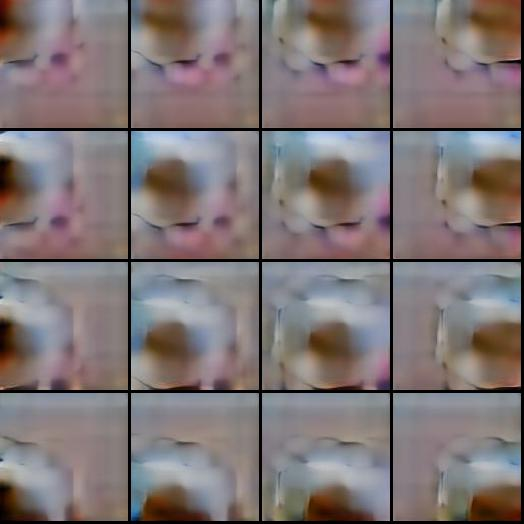
\includegraphics[width=0.3\textwidth]{figures/ptz/words_spatial}
        \label{fig:words-spatial}
    }
    \subfloat[][]{
        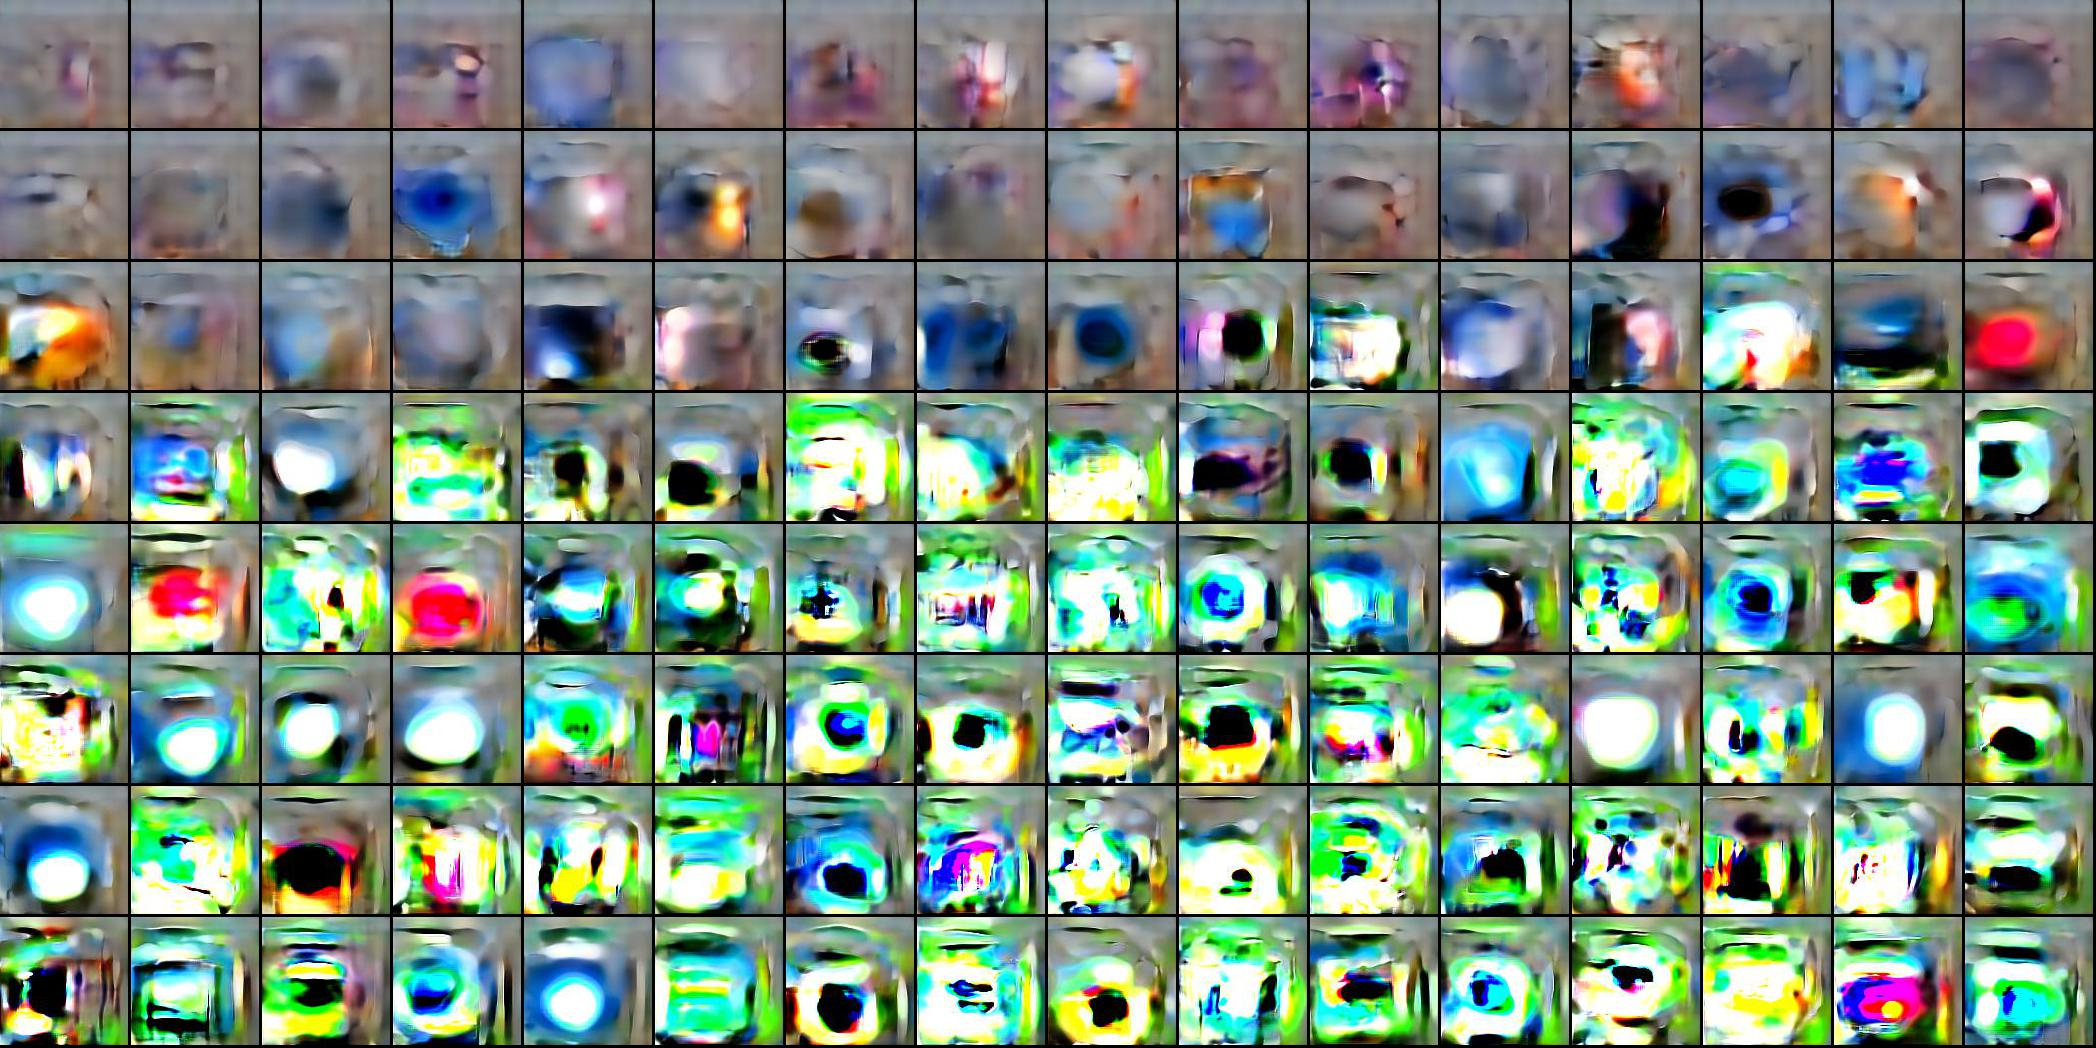
\includegraphics[width=0.6\textwidth]{figures/ptz/top_words}
        \label{fig:words-top}
    }
    \caption{CIB-AE decodings of single `words', \emph{ie.} one-hot encoding vectors. An image is reconstructed as a normalized word-histogram.
             \protect\subref{fig:words-spatial} 512 words are nearly duplicated at $4 \times 4$ positions within the image.
             \protect\subref{fig:words-top} The 128 most common words (shown in their center position).}
    \label{fig:cibae-words}
\end{figure}

Through the Dirichet priors on topics and topic-word distributions, LDA descendants such as the spatio-temporal topic model make the implicit assumption that documents have sparse word distributions. Although we do not specify exactly how sparse such a sparse mixture of sparse multinomials is, we have found in practice that simply renormalizing the features of conventional autoencoders produces word-distributions that are too uniform to be modelled productively by LDA. Therefore, CIB-AE employs an additional regularization term in its loss,
\begin{equation}
    L_{CIB} = -\log p(\mathbf{I} | \mathbf{\hat{I}}) - \lambda MI\left(\mathbf{I}, W\right)
\end{equation}
where $W \sim e(I)$ and $MI$ stands for the mutual information, a measure of the degree if dependence between two random variables. Choosing a large value for $\lambda$ will result in representations that favor high mutual information between images and encoding distributions, \emph{ie.} those where training images are as distinguishable as possible in encoding space. On the other hand, choosing a small $\lambda$ will result in encodings which may be very similar, but result in a low MSE. In other words this regularization term ensures that encoder collapse does not occur as it does with many other autoencoders. We note an interesting connection to the literature on VAEs, which uses an approximate prior $q(W|\mathbf{I}) \approx p(W)$. Rewriting $MI\left(\mathbf{I}, W\right)$ as $D_{KL}[(I,W) \| IW ]$, our objective and the VAE objective take extremely similar forms: In particular, $L_{CIB} = -\log p(\mathbf{I} | \mathbf{\hat{I}}) - \lambda D_{KL}[(\mathbf{I},W) \| IW ]$ while $L_{VAE} = -\log p(\mathbf{I} | \mathbf{\hat{I}}) + \lambda D_{KL}[q(W|\mathbf{I}) \| p(W) ]$.

To illustrate how our loss works, consider another way to rewrite the mutual information: $ MI\left(\mathbf{I}, W\right) = H[W] - H[W | \mathbf{I}] $ where $H[W | \mathbf{I}]$ signifies the conditional entropy. By subtracting the mutual information from the loss, the $H[W | \mathbf{I}]$ term ensures that individual encodings must have low-entropy, and are therefore sparse, while the $-H[W]$ term ensures that the overall distribution of encodings is high-entropy, and therefore as uniform as possible. The combination of these two terms means that the encodings must use different dimensions of the feature space from one another.

Reorganizing the mutual information in this also way reveals how to estimate it from a minibatch of size $M$:
\begin{equation}
\begin{split}
    -MI\left(\mathbf{I}, W\right) = H[W | \mathbf{I}] - H[W] = \\
    \mathbb{E}_{w \sim e(I)}\left[ -\log p(w) \right] - \mathbb{E}_\mathbf{I}\left[ \mathbb{E}_{w \sim e(I)}\left[ -\log p(w) \right] \right] \approx \\
    -\frac{1}{M} \sum_{m=1}^M \sum_{d=0}^V e(I_m)_d (\log e(I_m)_d) +
            \sum_{d=0}^V \overline{h}_d \log \overline{h}_d
    \end{split}
\end{equation}
where $\overline{h}$ signifies the average encoding for the $M$ images in the batch. Clearly, estimating an expectation over the space of all possible training images with a minibatch of few dozen or at most a few hundred examples is crude. Nevertheless, the terms of this approximation naturally fit our goal of producing maximally sparse, maximally distinct encodings for as much of the training data as possible. To summarize our approximation of the CIB loss
\begin{equation}
L_{CIB} \approx \mathcal{L}_{CIB} = \frac{1}{M} \left( \sum_{i=1}^M \frac{(I_m - \hat{I}_m)^2}{|I|}
                                    - \lambda \sum_{d=0}^V e(I_m)_d (\log e(I_m)_d) \right)+
                                     \lambda \sum_{d=0}^V \overline{h}_d \log \overline{h}_d
\end{equation}
where $|I|$ denotes the (fixed) number of pixel for an input image. In other words our loss is the MSE plus the average entropy of all encodings, minus the entropy of the average encoding. We find in practice that when the image space is normalized to the range $[-a,a]$, $\lambda = \frac{(2a)^2}{\log V}$ is a good choice, where $V$ is the dimension of the encodings \footnote{Note $\log V$ is the maximum possible entropy for a categorical distribution of dimension $V$, so this choice represents letting the MSE and MI terms have `equal' weight when both are in their worst cases}.

Our specific choice of architecutre is inspired by the feature layers of VGG \citep{Simonyan14c}. In particular, following the approach of Segnet \citep{BadrinarayananK15} we choose a VGG-like encoder, with a symmetric decoder of transposed convolutional layers. This style of encoder uses a sequence of convolution `blocks', which each ultimately either downsample (Max Pool) or upsample (Nearest Neighbor) the activations by a factor of two. We add an additional dropout and an additional softmax layer to the encodings to constrain the real-valued activations of a Segnet style encoding to a simplex. Our feature representation downsamples the image spatially by a factor of 32, while producing a 512 channel feature activation for each spatial region. All experiments are conducted with $128 \times 128 \times 3$ input images, resulting in $4 \times 4 \times 512 = 8192$ dimensional encodings distributions. The full details of our architecture are found in App.~\ref{ch:cibae-arch}, however we emphasize that by adding these two extra layers and the additional loss term, our approach can be transferred to many domains and existing autoencoder architectures.

\section{Spatial topic prediction model}

Beyond simply finding any low-dimensional representation of the image space a PTZ camera may encounter, the spatio-temporal topic model is able to learn such a representation that is also spatially coherent. We situate the topic model's neighborhoods in the space of views, meaning that the resulting learned topic priors will form a map of the visually distinct regions in pan-tilt-zoom space.

Because our model is designed to make the topic priors locally smooth, we are able to develop a simple spatial prediction scheme for topic priors. Our spatial prediction model is fast to fit and run online, taking camera pose, learned topic prior pairs as training data, and predicting the topic prior for a test pose. We take inspiration from a nearest-neighbor model: in the simplest case our approach is to predict the topic prior of the nearest training point for a test point. However, we envision using this system with only a few dozen training points, and would prefer predictions to degrade towards the global average topic distribution than a poor estimate of the topic prior when the test point is not near any training point.

To achieve this property, we implement our predictions using an energy-based model, using a weighted sum over the topic distributions we have observed so far, where far training points have low weight and near training points have high weight. Rather than performing such a prediction with a direct mixture of observed topic-priors and renormalizing, we choose to implement the weighted sum in terms of the log-probability of each training topic, and then use a softmax to return to the natural probability space. Note that if the mixture of log-probabilities belongs to a valid probability distribution (\emph{eg.} all the weight is placed on a single training point), the softmax function returns exactly that distribution.

We define the weights in terms of a Boltzmann distribution (\emph{ie.} the softmax of negative energy), using the distance to each observed topic prior as the energy. Let $D_X(x)$ denote the distance vector from point $x$ to each point in the training set $x_i \in X$. This choice of weight function has the appealing property that if any entry of $D_X(x)$ is much smaller than the rest, all of the weight will be put on that training point. Further, with this weight function, by controlling the scale of the distances we can control the sparsity of the weight vector; when the average distance is low the weights will be fairly uniform, while when the average distance is high, the weights will be sparser. We choose to use the plain $\mathit{L}_2^2$ distance between pan-tilt-zoom points as our distance function. However, in order to appropriately scale the distances and balance dimensions which may not truly incur equal loss of relevance for higher distances, we first scale the input points by the vector $w$ \footnote{Our distance could also be called a Mahalanobis distance (normally formualted in terms of the covariance matrix $\Sigma = ww^T$)}. To summarize our prediction model, given $N$ training points $X$ each paired with an observed topic prior in $\Theta_X$:
\begin{equation}
\begin{split}
    D_X(x) = 
    \begin{bmatrix}
    \|w^Tx - w^T x_1 \|_2^2, & \|w^Tx - w^T x_2 \|_2^2, \ldots, \|w^Tx - w^T x_N \|_2^2
    \end{bmatrix}\\
    W(x) = \sigma \left( -D_{X}(x) \right)\\
    \theta(x) = \sigma \left( W(x) \log \left(\Theta_X \right) \right)
\end{split}
\end{equation}

Finally, we note that setting $w$ by hand is difficult as the best choice may vary from environment to environment, and is unnecessary, as both fitting and prediction are extremely efficient with this model. Instead, given a validation set of size $X^\star, \Theta^\star$ held out of training, we consider the information lost by using our model, measured by the mean Jensen-Shannon Divergence on the validation set:
\begin{equation}
L_w = \frac{1}{|X^\star|} \sum_{x \in X} D_{JS}\left[\theta(x) \| \Theta^\star_x \right]
 =  \frac{1}{|X^\star|} \sum_{x \in X} \frac{1}{2} \left(D_{KL}\left[\theta(x) \| m(x) \right] + D_{KL}\left[\Theta^\star_x \| m(x) \right]\right)
\end{equation}
where $m(x) = \frac{\theta(x)+\Theta^\star_x}{2}$. While $D_{KL}$ would most directly measure the information lost by approxmating the true topic distribution with the prediction, $D_{JS}$ is additionally symmetric, positive, and bounded above, making it a more convenient loss function. In addition, this loss and our model are differentiable, so we are able to fit $w$ using gradient descent and a 2-fold cross-validation procedure. As a final note, although a more complex distance model may better match how topic-priors are spatially distributed, because we aim to train this model with only a few dozen examples we prefer a simpler model that is less prone to overfitting.

\section{Experiments}

\subsection{Simulated Pan-Tilt-Zoom Camera Dataset}
\begin{figure}
    \centering
    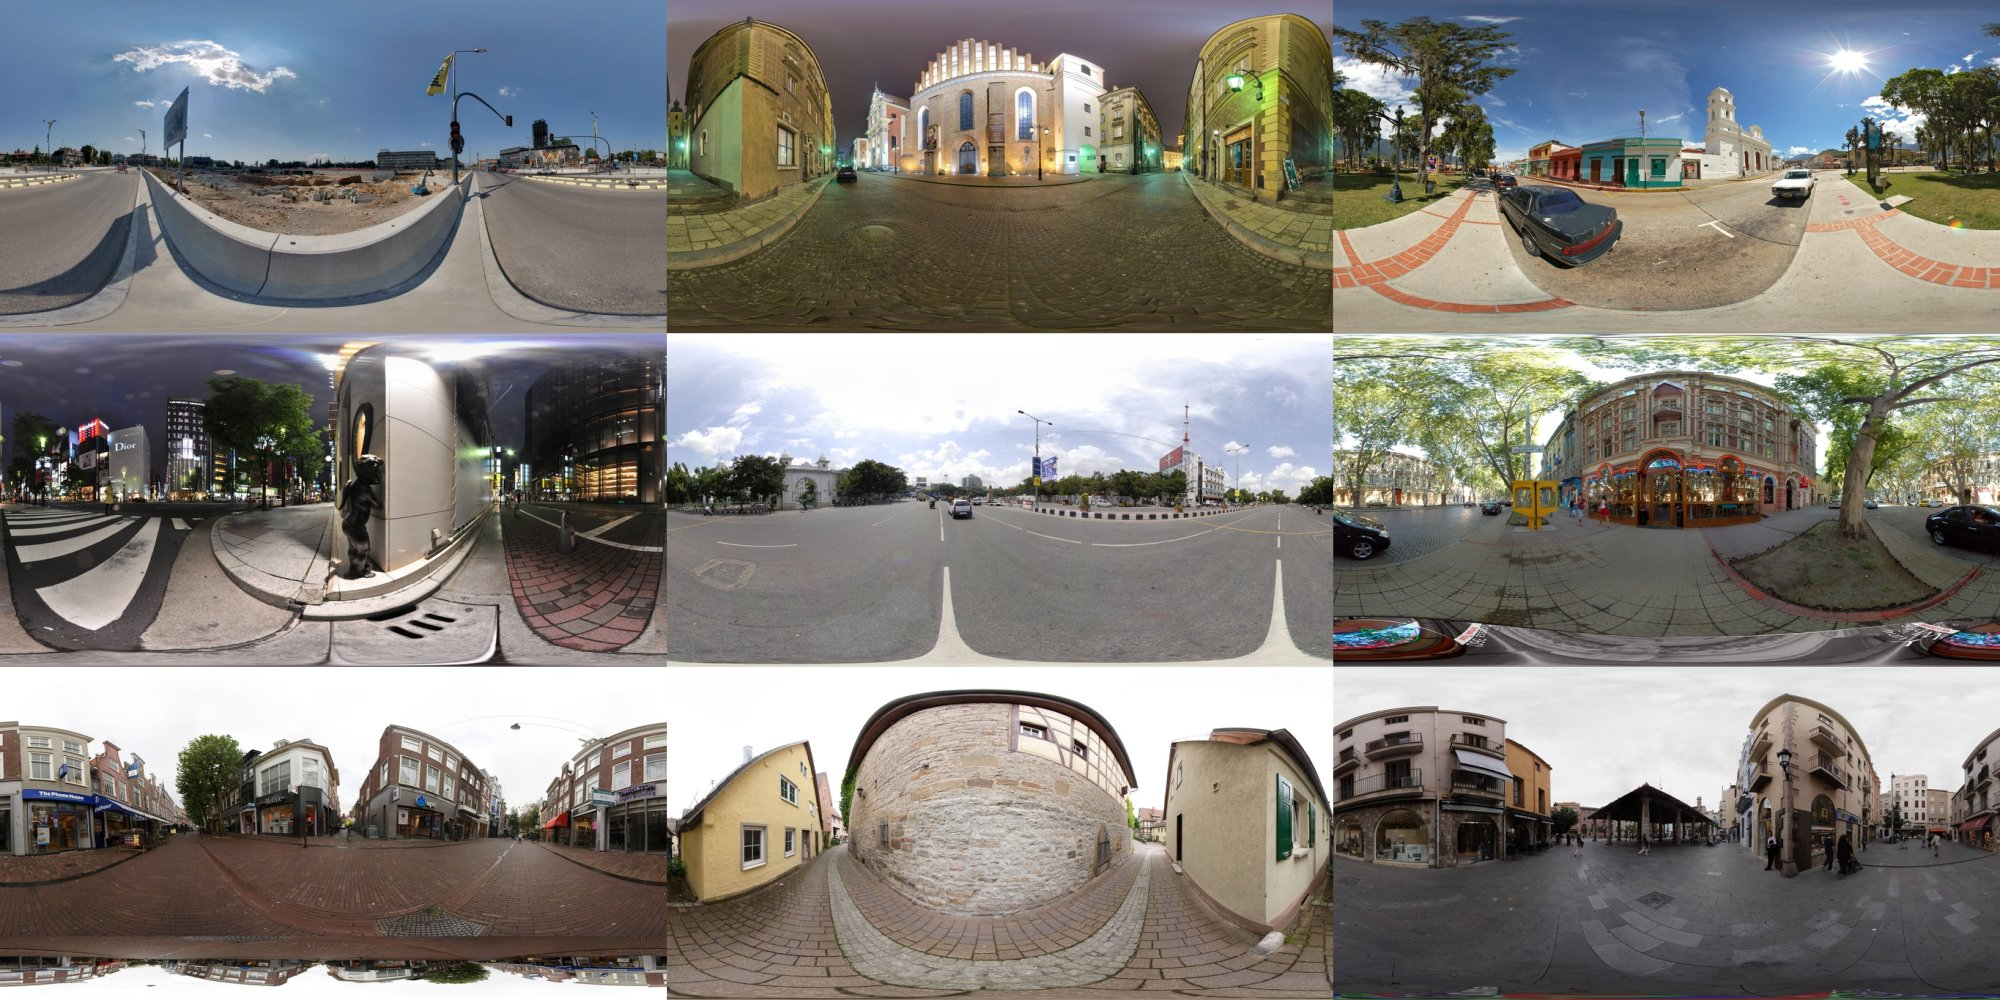
\includegraphics[width=0.85\textwidth]{figures/ptz/sun360_9x.jpg}
    \caption{Example 360 degree panoramas from the SUN360/street dataset.}
    \label{fig:sun360_ex}
\end{figure}

We demonstrate our approach with a simulated outdoor pan-tilt-zoom camera, using data from the `street' category of the SUN360 dataset \citep{SUN360}. Specifically SUN360/street comprises a dataset of 161 360 degree panoramas projected into rectangular $9104 \times 4552$ pixel images (Fig.~\ref{fig:sun360_ex}). These panoramas are taken in various cities and towns across the world, from street corners and from car-mounted cameras. We parameterize views in terms of tilt angle $T$, pan angle $P$, zoom factor $Z$. Given a base field-of-view (fov) $A_0$ and a target camera resolution, we compute the projection to the desired perspective $R = R_TR_P$ where
\begin{equation}
\begin{split}
R_T =& 
\begin{bmatrix}
1 & 0 & 0\\
0 & \cos(T) & -\sin(T)\\
0 & \sin(T) & \cos(T)
\end{bmatrix}\\
R_P =&  
\begin{bmatrix}
\cos(P)        & \sin(P) - \sin(T)            & \sin(P)\cos(T)\\
\sin(P)\sin(T) & \cos(P)\cos(T)^2(1 -\cos(P)) & \cos(T)\sin(T)(1-\cos(P))\\
\sin(P)\cos(T) & \sin(T)\cos(T)(1-\cos(P))    & \cos(P)+\sin(T)^2(1-\cos(P))
\end{bmatrix}
\end{split}
\end{equation}
Using the fov $A = A_0/Z$ and output image resolution, we represent the output pixel locations as pan-tilt rotations from the center $P$, $T$. Then, projection proceeds as rotation by $R$ and a lookup in the full panorama image for each pixel in the output image. In all our experiments we consider a base fov of 76 deg and zoom factors $Z \in [1, 12]$, similar to a standard commodity camera. Further, to avoid wrapping angles, we consider only $T \in [-60, 60]$ and $P \in [-120, 120]$ degrees (SUN360 is designed so that the horizon is horizontal and vertically centered in all panoramas).

\subsection{Place-specific autoencoder}

A key advantage of the topic-model based approach is that it can be trained online, whereas this is not practical for large deep-networks. This means that rather than learning a single model which aims to produce a low-dimensional embedding of all possible images, our robotic camera system can learn a new, place specific model, and is thus required to represent a vastly simpler space of images.

Our approach delegates learning the globally-salient image embedding to the CIB-AE. In particular, we trained our feature model using epochs of 5000 random views from 80 random SUN360/street panoramas. We found that choosing a new set of random training views for each epoch was crucial, however we kept the validation set fixed throughout training. The projection described in the previous section is time consuming for high-resolution images, especially for those that do not fit in GPU memory. Therefore we trained for 175 epochs on random square crops from the warped panorama images, and then 25 more epochs on projections to fine-tune the results. We achieved our results using the adaptive learning rate optimizer Adam~\citep{KingmaAdam}, however found that a learning rate decay by a factor of 0.9 every 10 epochs was also necessary. Example input images and their autoencoded counterparts can be seen in Fig.~\ref{fig:cibae_encodings}. We found the mean entropy of image encodings from 1000 random views from the test set to be 6.170 nats \footnote{While bits is the unit for information measured by entropy using $log_2$, nats is the unit when the entropy is calculated using $ln$}, or approximately equivalent to a uniform PMF over just 470 dimensions. On the other hand, the entropy of the mean encoding distribution from these 1000 examples was 8.192 nats, whereas the maximum possible entropy where all feature dimensions were used uniformly would have had an entropy of 9.011 nats.

\begin{figure}
    \centering
    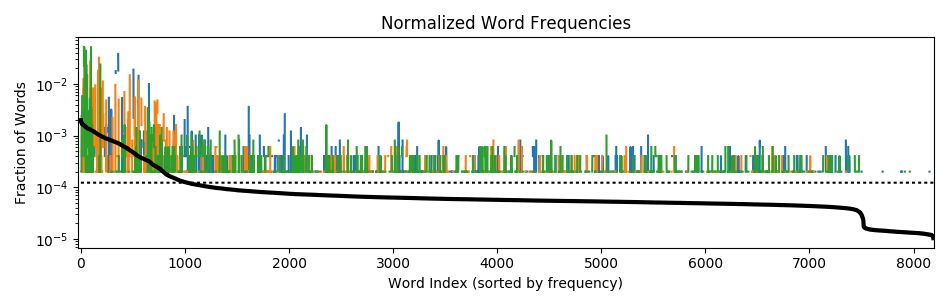
\includegraphics[width=0.95\textwidth]{figures/ptz/word_frequency}
    \caption{Word-distribution, sorted by frequency, of the average encoding over 1000 test images (heavy black line) and normalized
             word-histograms for 3 random images (colored lines). A uniform histogram over the 8192 dimensions (dashed black line) represents the ideal average encoding and the worst-case individual encoding.}
    \label{fig:cibae-words-distribution}
\end{figure}

\begin{figure}
    \centering
    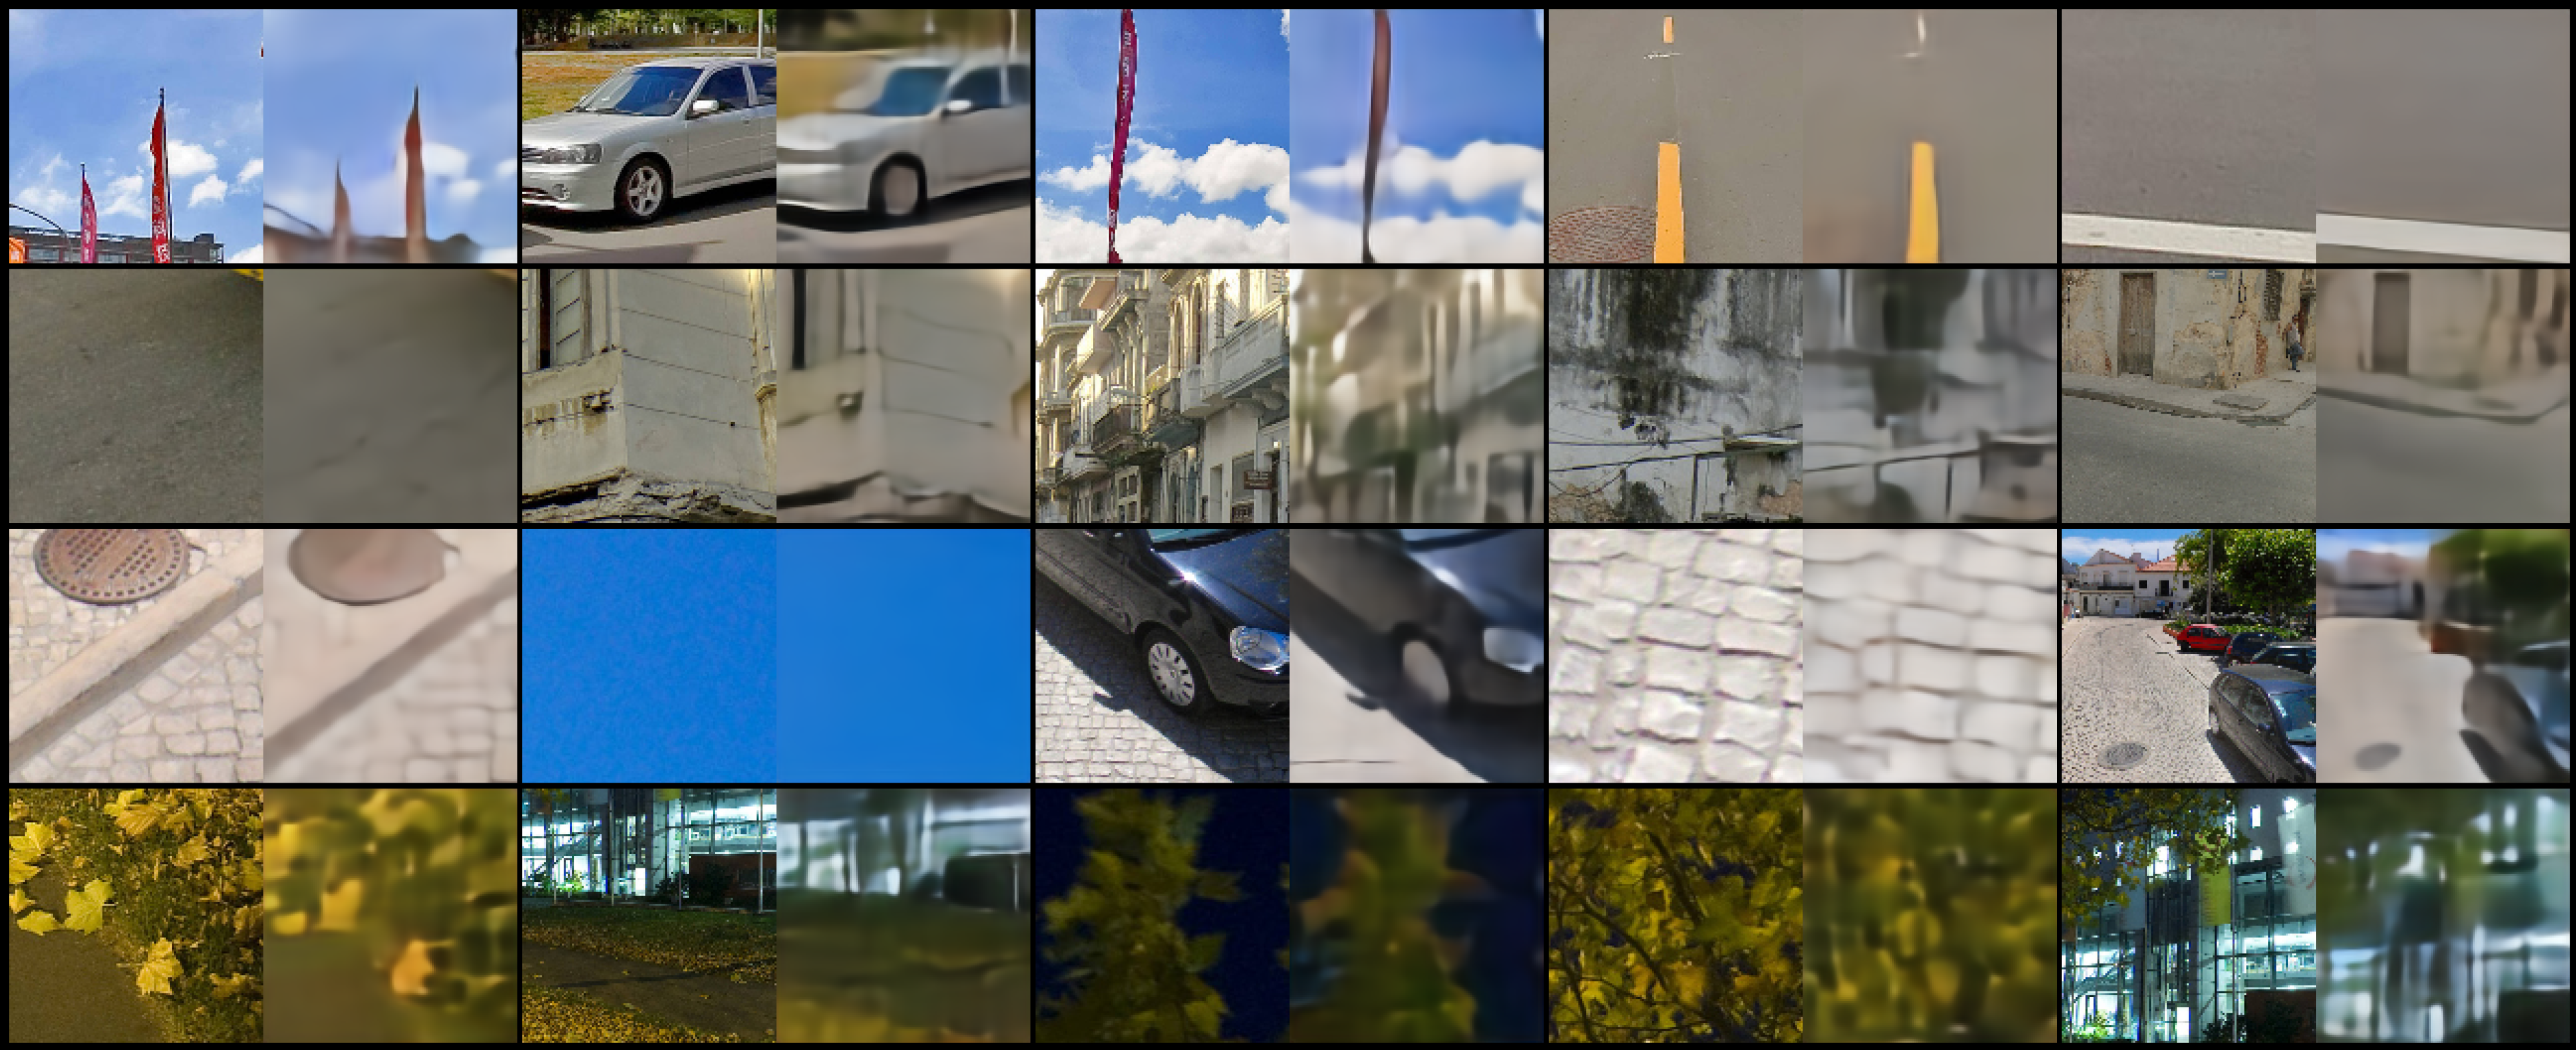
\includegraphics[width=\textwidth]{figures/ptz/mc3ae_encodings}
    \caption{Random example input images (left) and CIB-AE reconstructions (right) for 4 worlds (rows) from the SUN360/street test set.}
    \label{fig:cibae_encodings}
\end{figure}

We train our view-predictor by alternating between observing new encoding distributions and refining a spatio-temporal topic model for a fixed period of 1 second. At the end of each refinement phase the spatial topic map is refit using normalized pan, tilt, and zoom-factor spatial coordinates and a corresponding point-estimate of the posterior for $\Theta$ given the topic assignment counts. Then, the partially trained spatial topic-prior map can be used to select the next training view (discussed in Sec.~\ref{sec:active-learning}) or it can be chosen uniformly at random.

When the image corresponding to the new view is extracted its word distribution is computed based on our trained CIB-AE. Because our Gibbs sampling inference method samples from the posterior for the topic assignment of a single word given all the others, it is necessary to discretize the encoding distribution rather than work with it directly. Note that despite an encoding dimension of 8192, it is possible to use a relatively small number of discrete observations without losing detail because individual images have low entropy encodings. In our experiments we define a constant `document' size of 2000 words per image; initial experimentation showed some degradation of performance below this level and little improvement above, however clearly the document size defines a tradeoff between the required number of sampling iterations and the amount of detail modelled.

We choose a spatio-temporal topic model with $K = 25$ topics and neighborhoods of size 10 degrees $\times$ 20 degrees $\times$ 6 (tilt $\times$ pan $\times$ zoom). This neighborhood size choice corresponds to the intuition that environments are semantically `smoother' in pan than tilt, and much smoother while zooming than moving the camera. We chose concentration parameter values $\alpha = 0.2,~\beta = 0.2$. We performed extensive cross validation to select these hyerparameter values values and certain other choices were found to perform much better for particular environments, however we did not find a combination of hyperparemeter values that was definitively much more performant than the others on average.

\subsection{Spatio-Semantic Image Encoding Results}

Since we aim to demonstrate a real-time system that can learn about its surroundings relatively quickly, we stop learning after 50 observations. As a first inquiry into what the model has learned, we directly decode the point estimates of the topic distributions $\hat{\Phi}$ by passing them through the CIB-AE decoder (See Figs.~\ref{fig:pano-0-topics},\ref{fig:pano-1-topics},\ref{fig:pano-2-topics}). Most other applications of visual topic models employ non-invertible feature functions and choose to inspect topics by looking at the most representative training images. To our knowledge, this is the first application of a visual topic model where the topics can be fully decoded and inspected directly as images. Interestingly, we find that for our autoencoder network, sparser encodings produce clearer images, while more uniform encodings produce muddled, mostly gray, blurry images. This motivates us to use a \emph{maximum a posteriori} (MAP) point-estimate for $\hat{\Phi}$ (and in the subsequent section $\hat{\Theta}$)
\begin{equation} \label{eqn:map_thetaphi}
\begin{split}
\hat{\Theta}_{g(x), k} =&
    \begin{cases}
        \frac{N^k_{g(x)} + \alpha - 1}{\sum_{j=1}^K N^j_{g(x)} + \alpha - 1} & if~N^k_{g(x)} > 0 \\
        0 & otherwise
    \end{cases} \\
\hat{\Phi}_{k, w_i} =&
    \begin{cases}
        \frac{N^{w_i}_k + \beta - 1}{\sum_{v=1}^V N^v_k + \beta - 1} & if~N^k_{g(x)} > 0 \\
        0 & otherwise
    \end{cases}
\end{split}
\end{equation}

\begin{figure}
    \centering
    \subfloat[][]{
        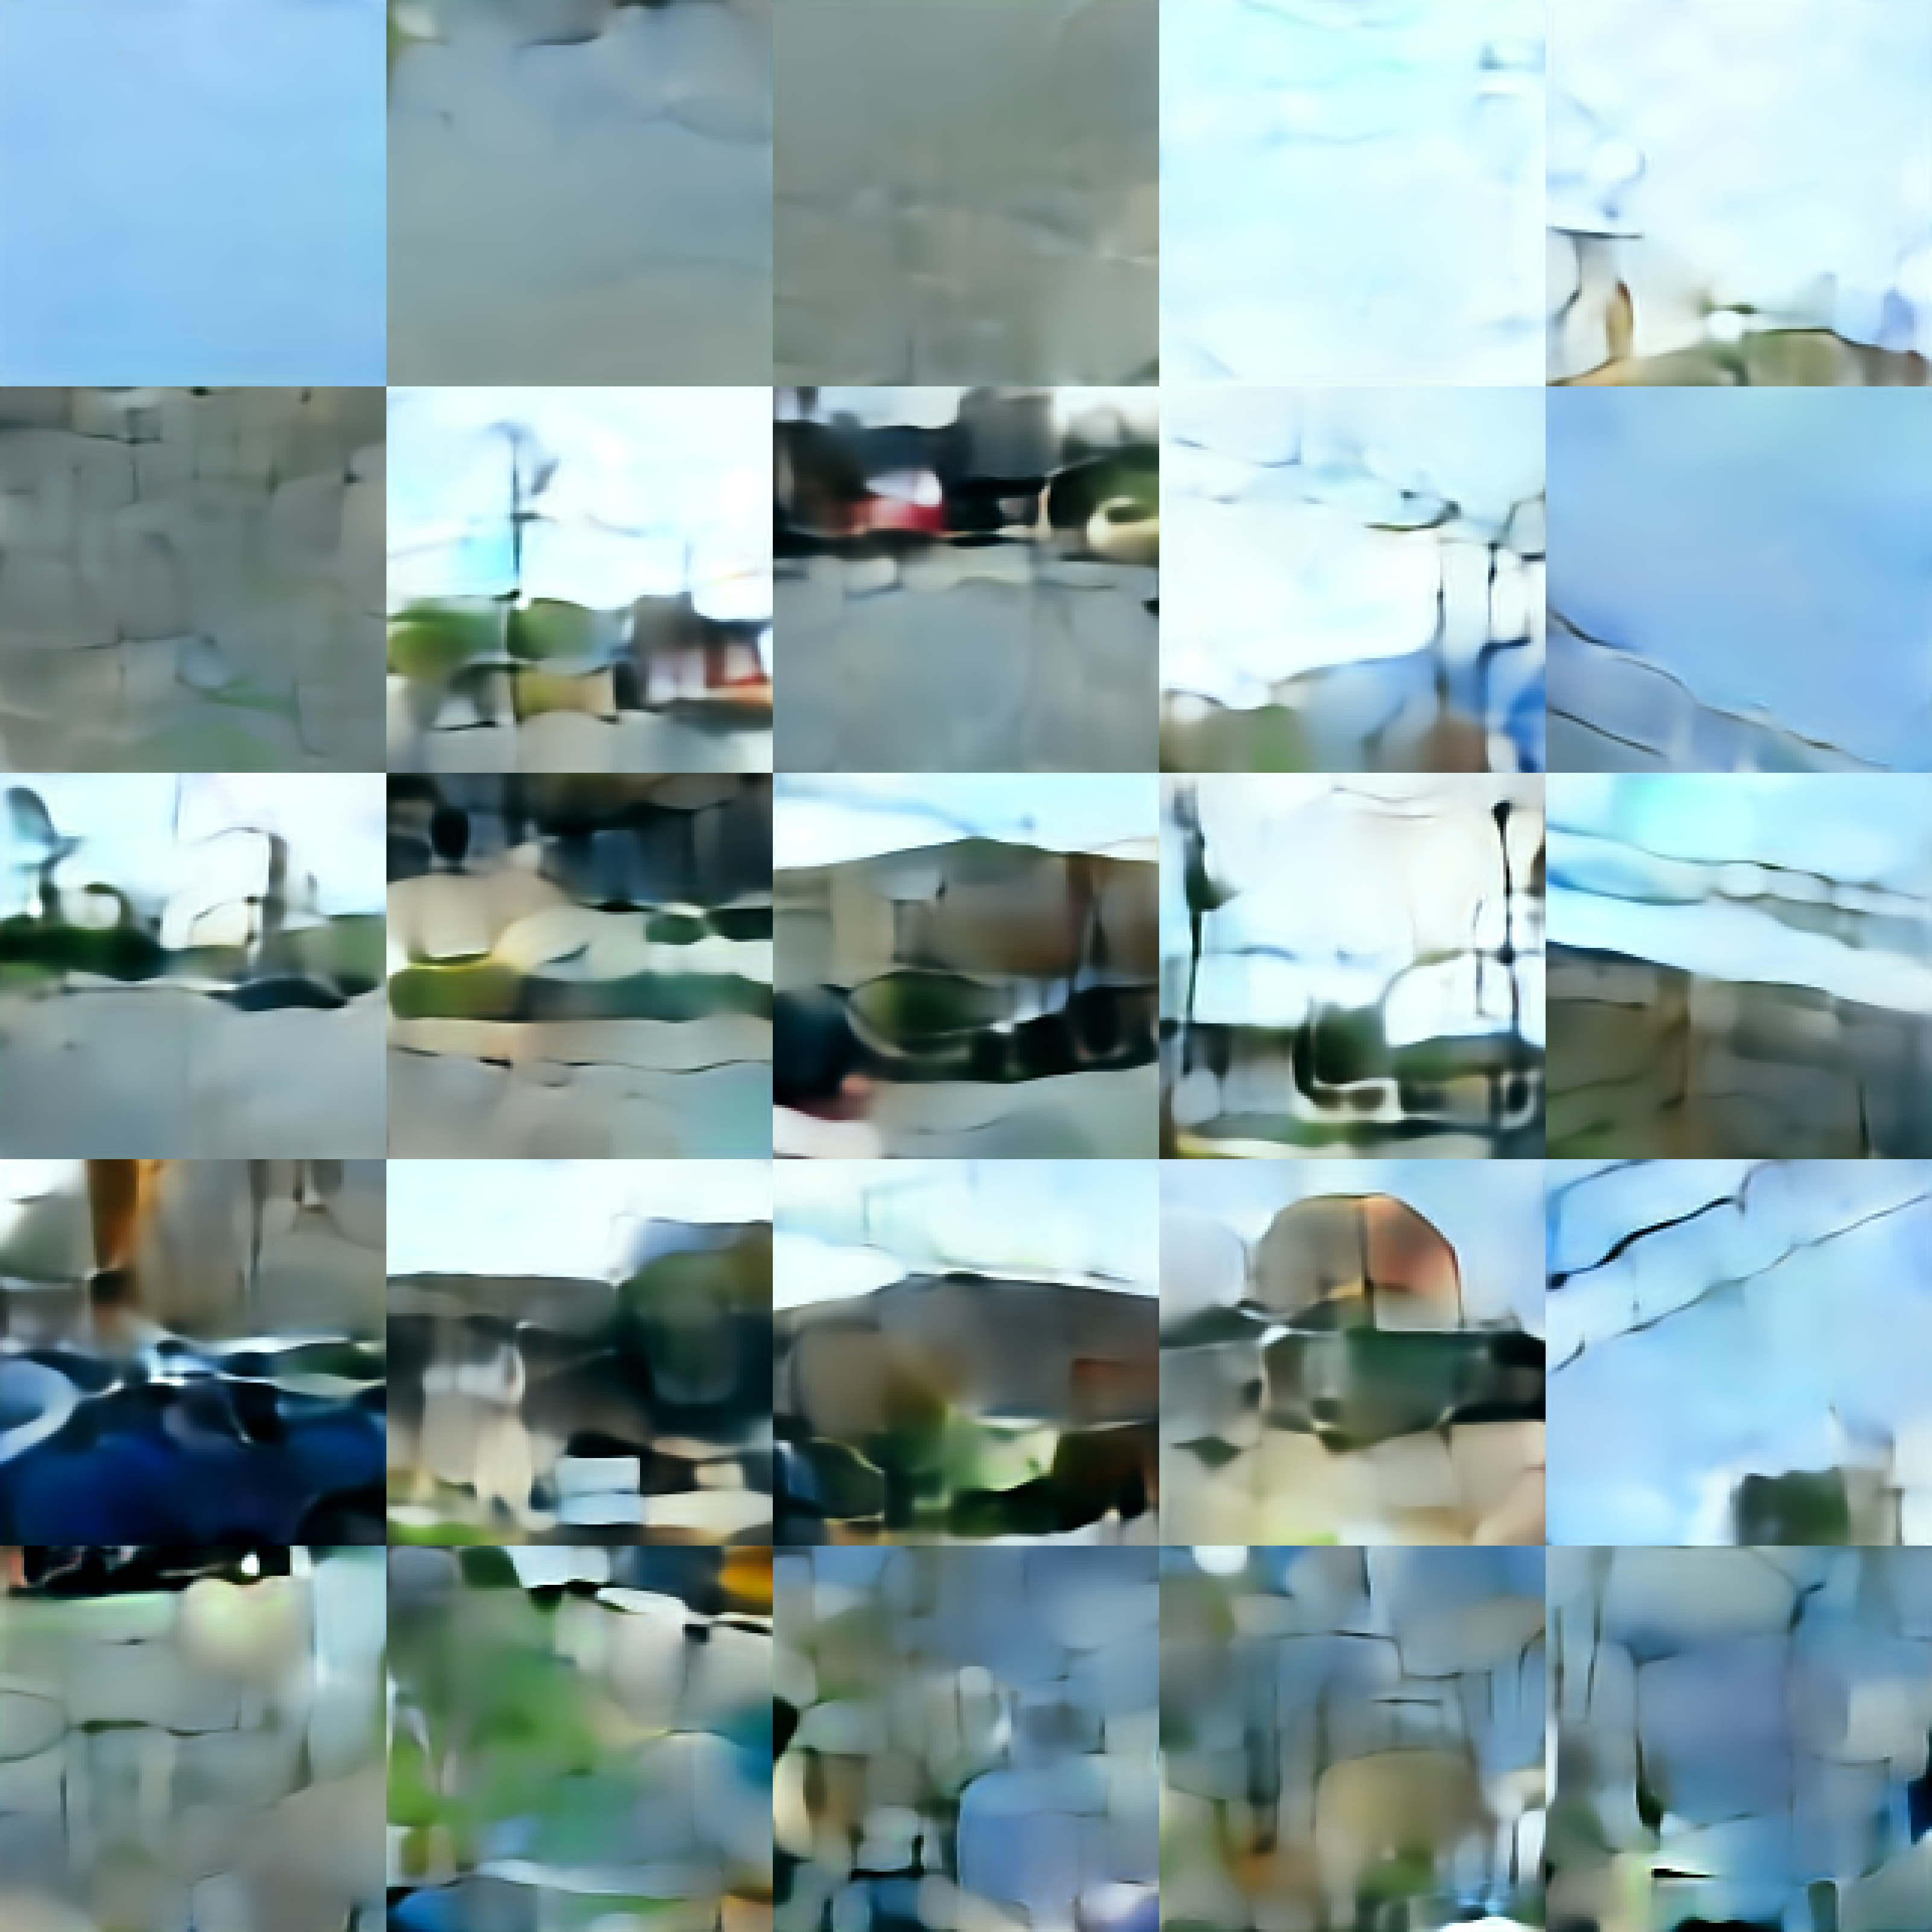
\includegraphics[width=0.4\textwidth]{figures/ptz/map_topics.png}
        \label{fig:map_topics}
    }
    \subfloat[][]{
        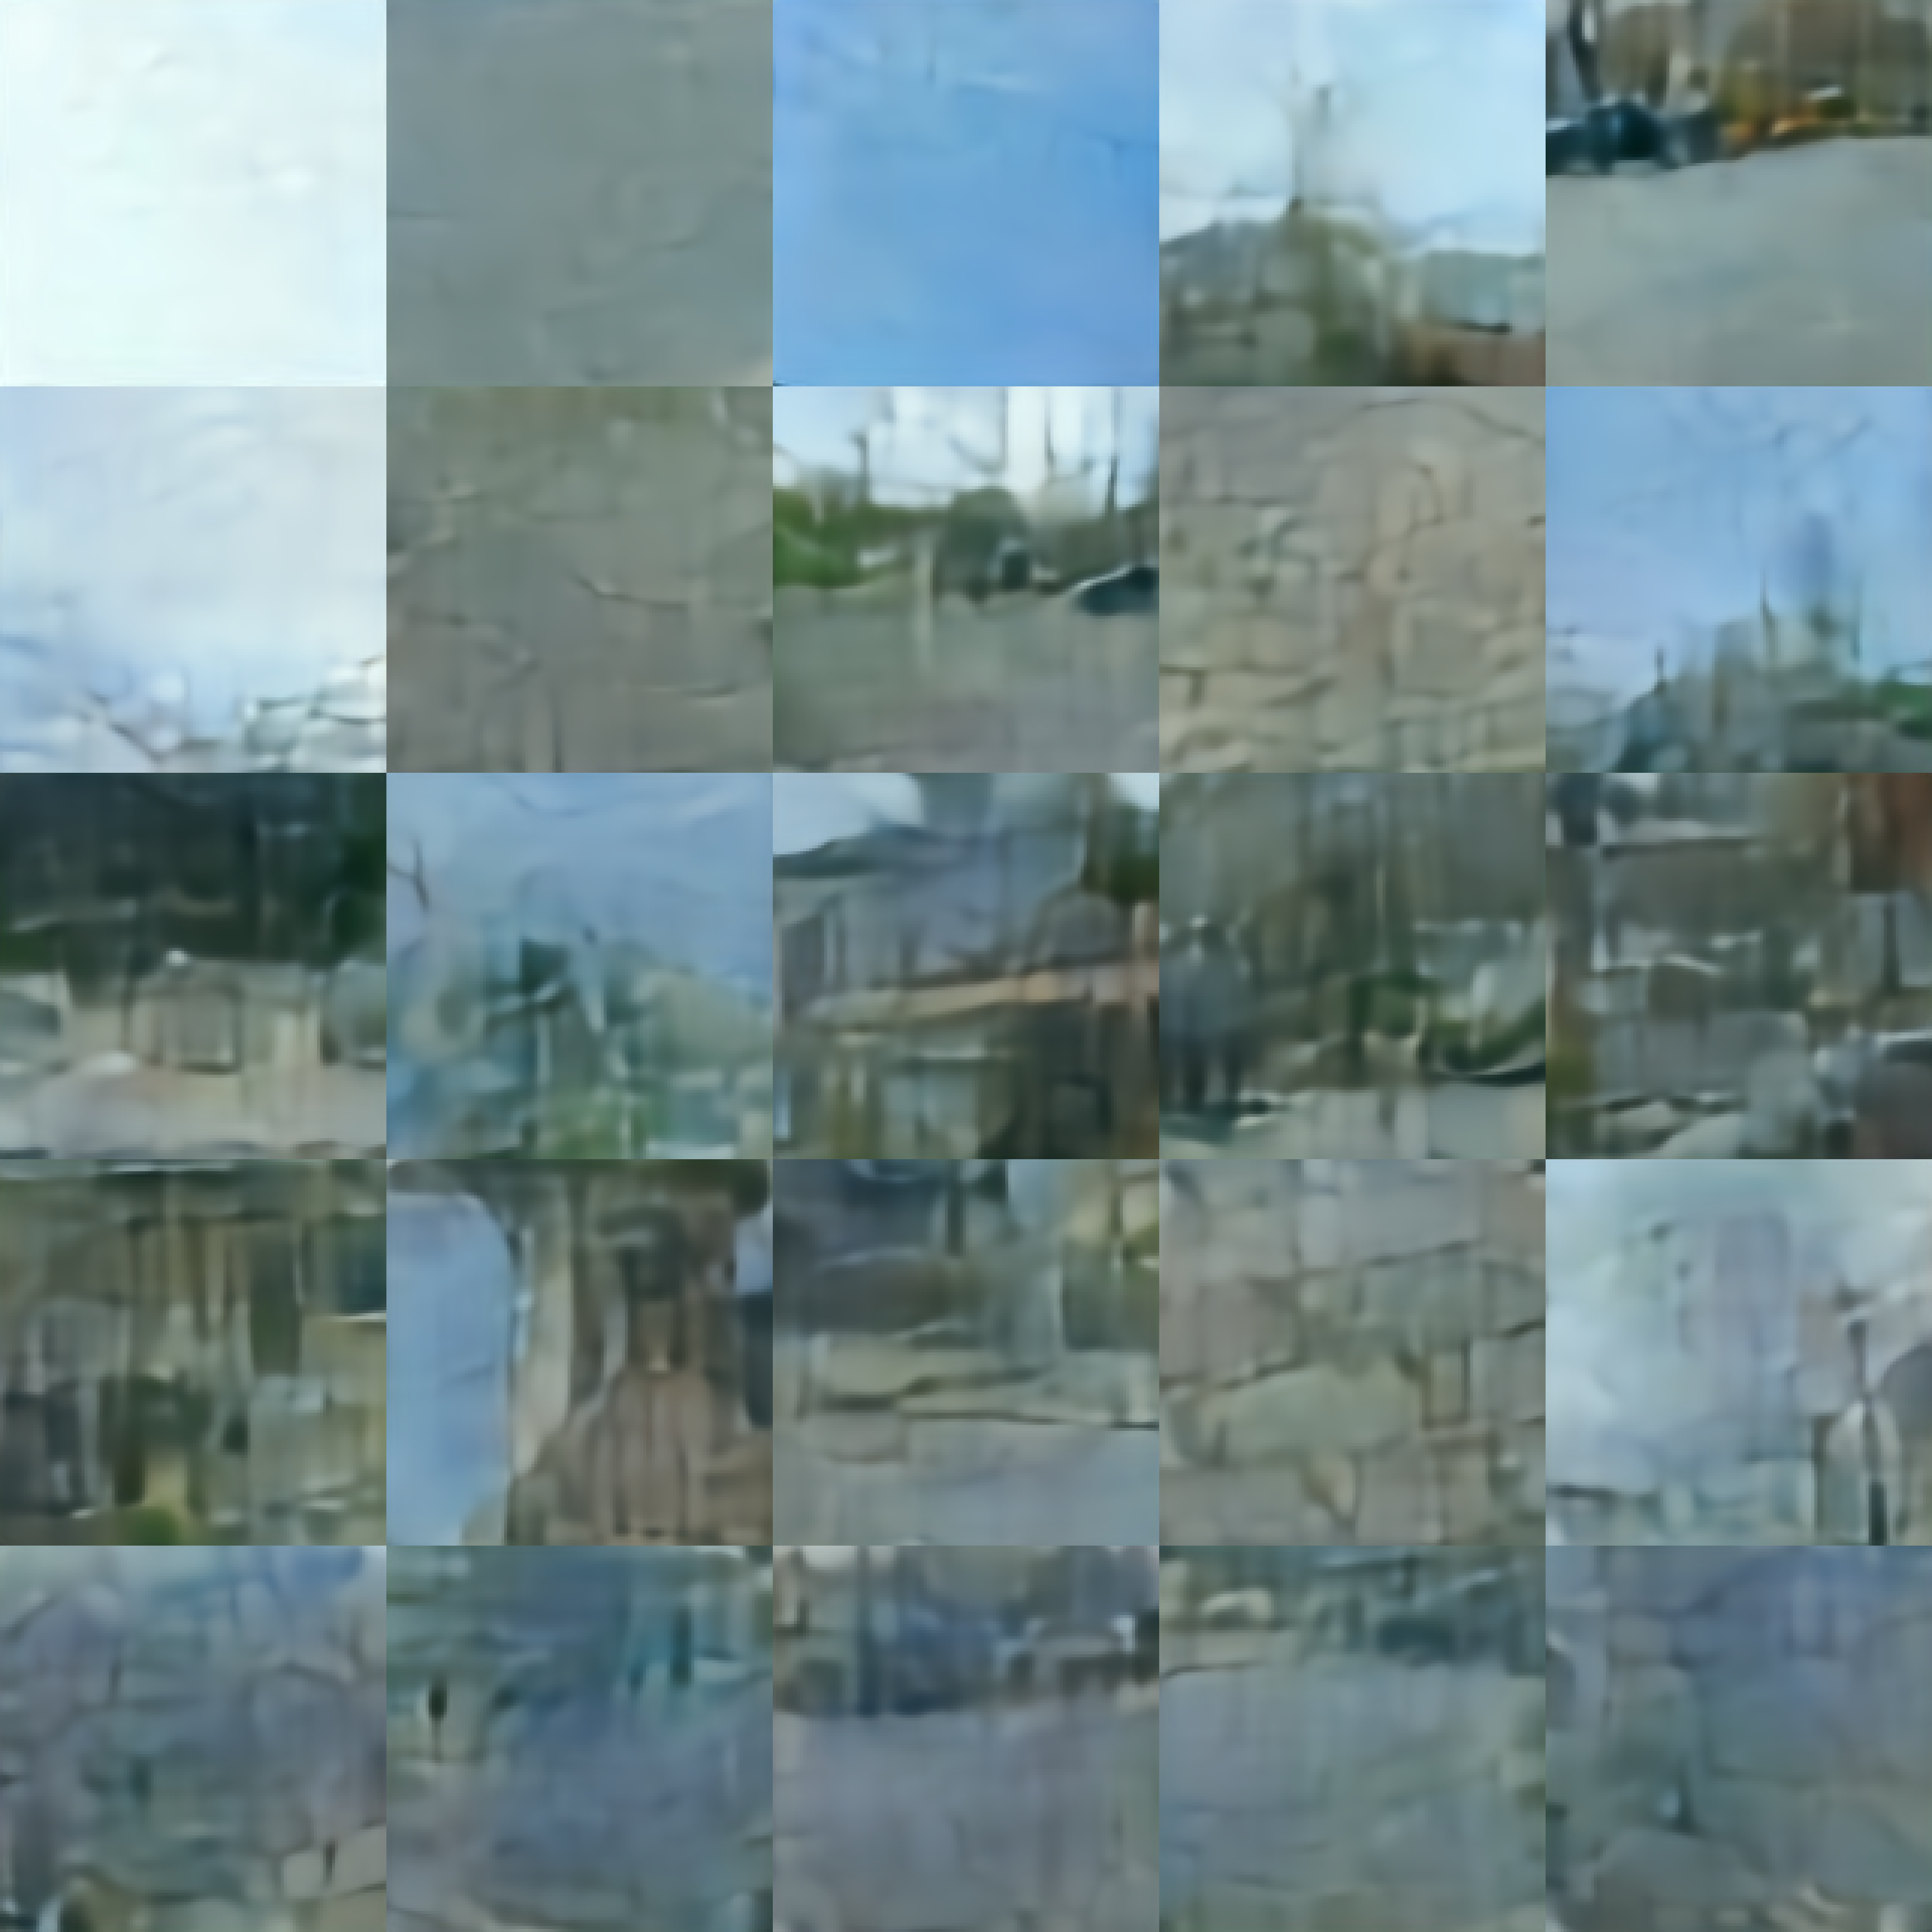
\includegraphics[width=0.4\textwidth]{figures/ptz/mle_topics.png}
        \label{fig:mle_topics}
    }
    \caption{MAP \protect\subref{fig:map_topics} vs MLE \protect\subref{fig:mle_topics} point estimates for $\Phi$ trained with identical datasets, directly decoded as images. Note that the MAP estimate features more distinctive topic images.}

\end{figure}

Prediction with our spatial topic prior model is extremely efficient, so we predict the topic priors for 10,000 random $P,T,Z$ views. In Figs.~\ref{fig:pano-0-map}, ~\ref{fig:pano-1-map}, and ~\ref{fig:pano-2-map} we present the resulting topic prior maps (one scatter plot per topic, in the same arrangement as the topic images), with the point $x_i$ omitted for topic $k$ if $\theta(x_i)_k < 0.01$, blue indicating $\theta(x)_k = 0.01$ and red $\theta(x)_k = 1$. Together, the decoded topics and view-topic maps provide an evocative graphical representation of how low-level textures combine into a higher level scene structure. After training, we collected 50 more views along with their inferred MAP topic priors (without performing any more refinement of $\Phi$). Among these observed views for each of the 35 test panoramas, we found $D_{JS}[\theta(x), \hat{\theta}]$ to be 0.1953 nats, while $D_{JS}[\mathrm{Unif}(K), \hat{\theta}]$ was on average 0.4122 nats\footnote{Recall $0 \leq D_{JS} \leq \ln(2) \approx 0.6931$}. This indicates that the topic mapping procedure is imperfect as is expected because of its weak geometric assumptions, nevertheless that it is better than a trivial strategy.

\begin{figure}{}{}
    \centerline{
    \begin{minipage}{0.6\textwidth}
        \subfloat[][]{
            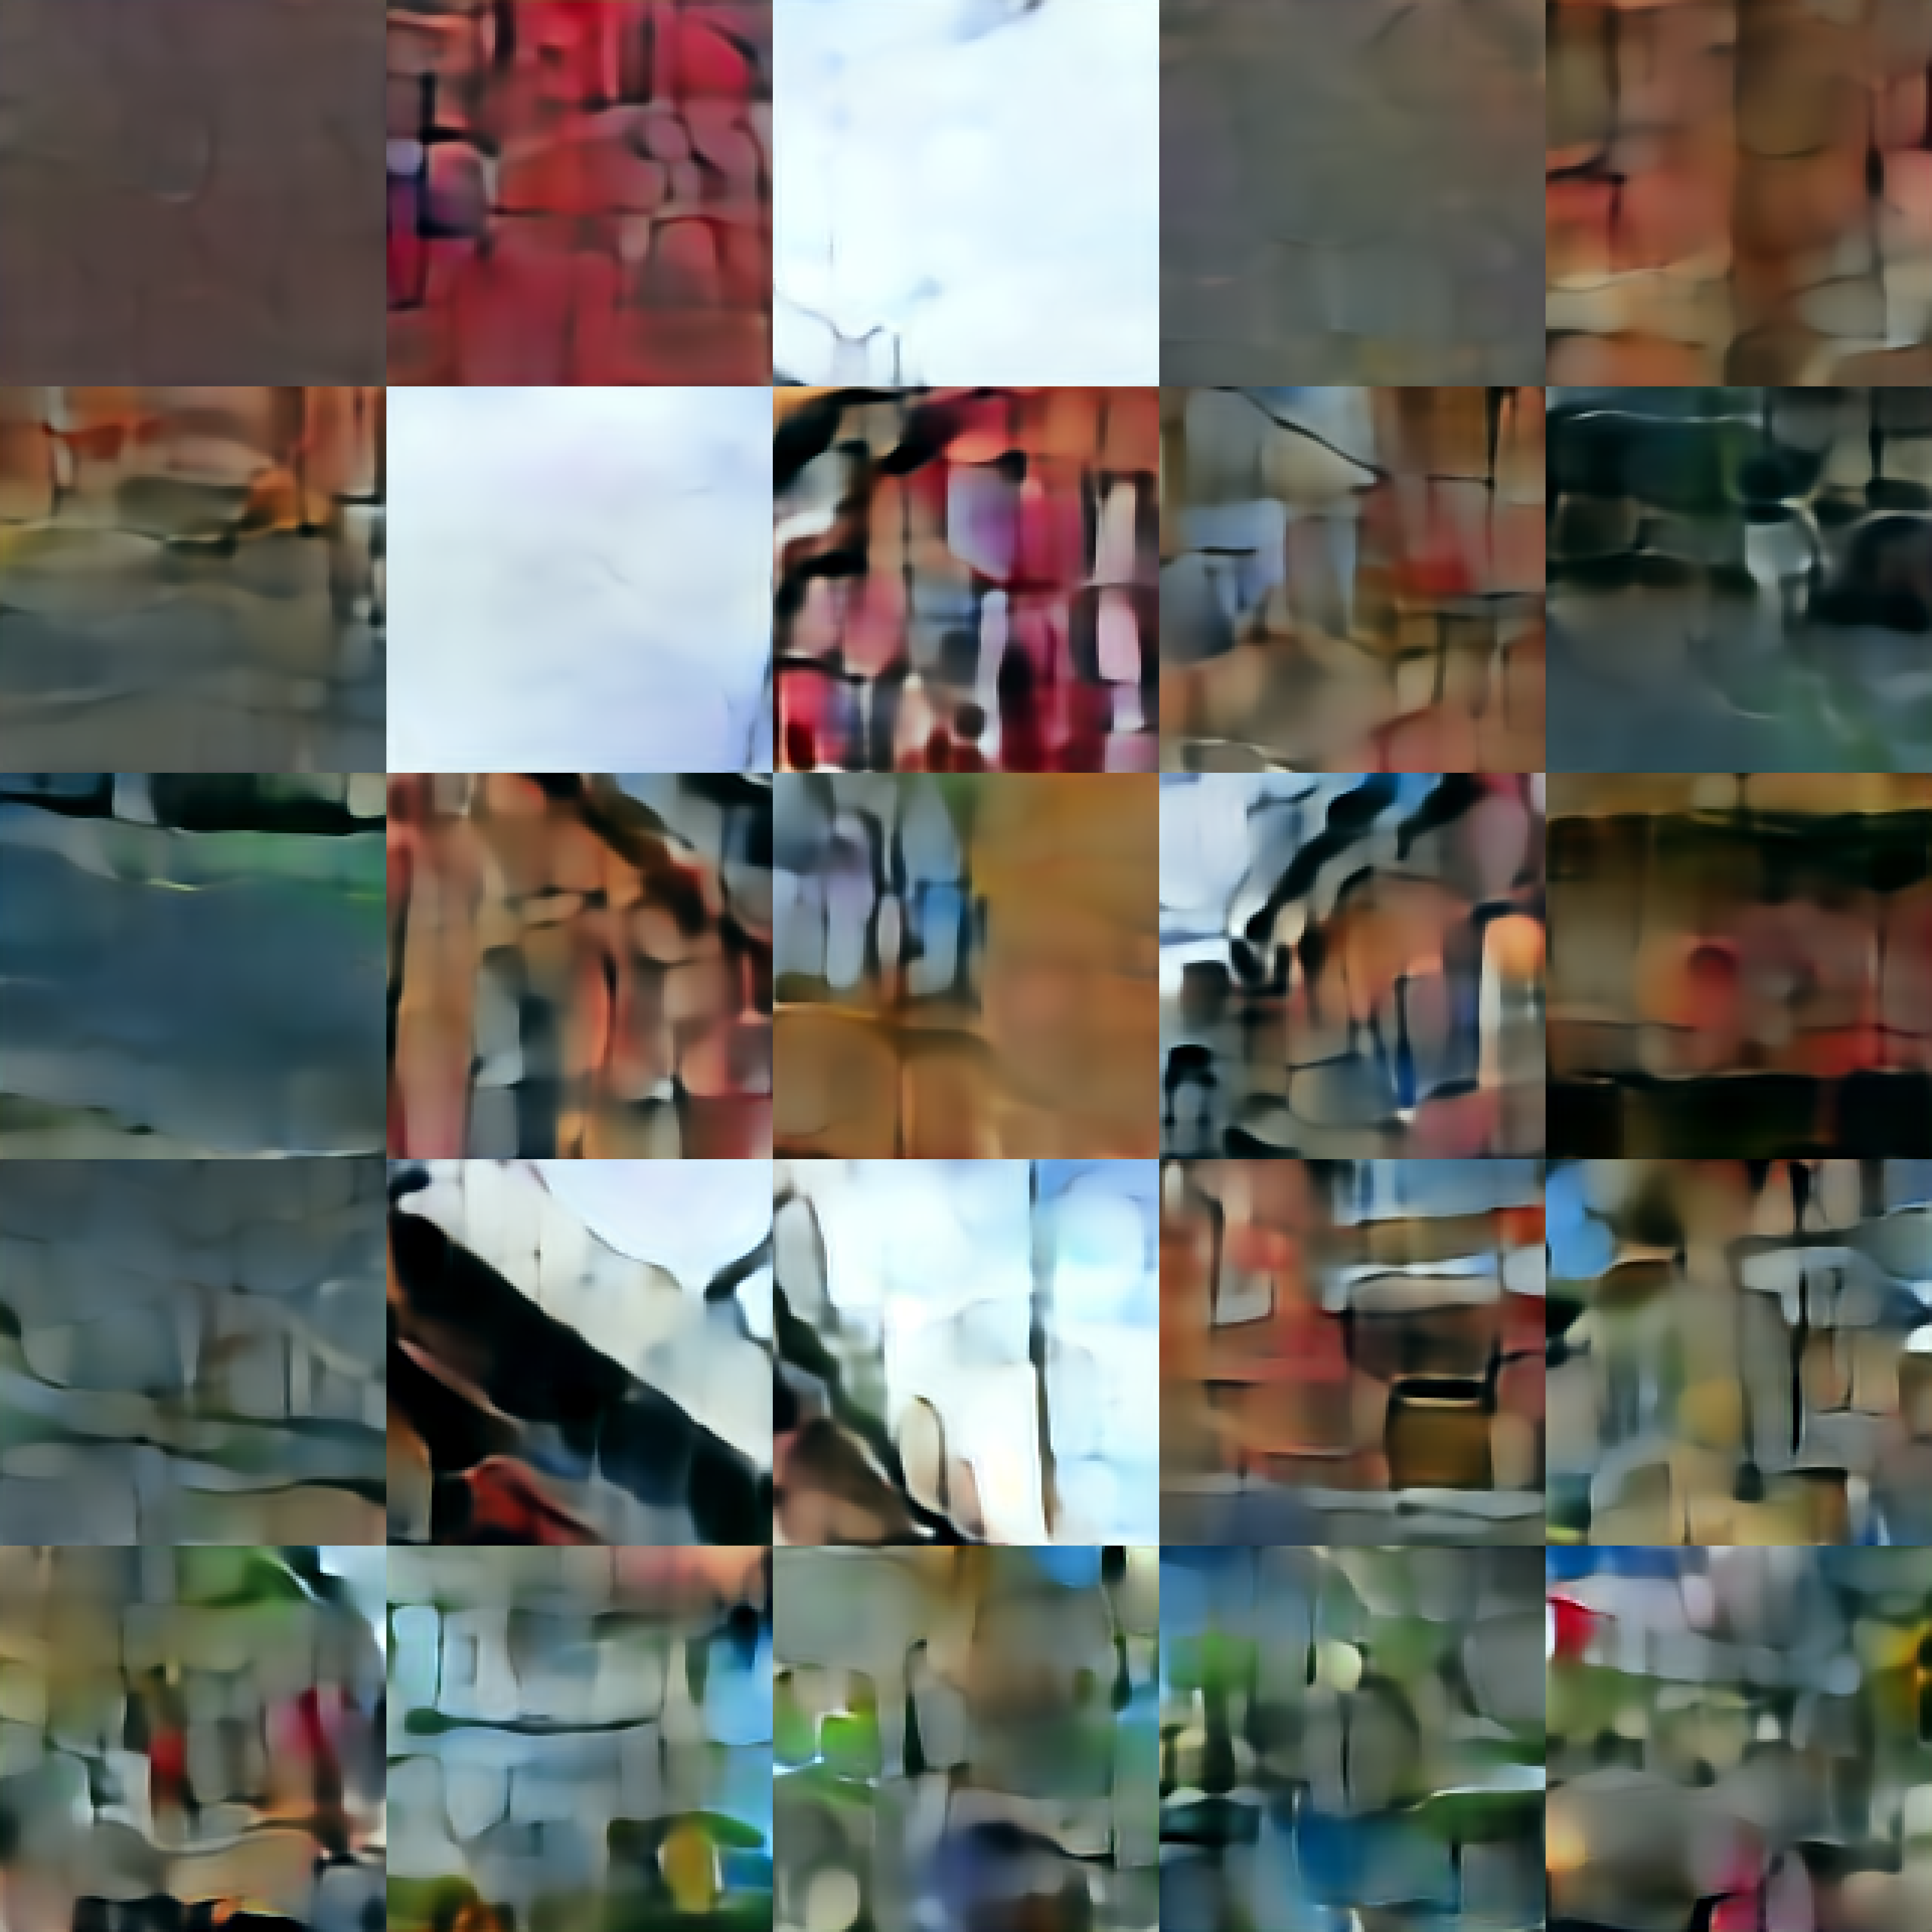
\includegraphics[width=\columnwidth]{figures/ptz/pano_0_topics.png}
            \label{fig:pano-0-topics}
        }
    \end{minipage} \hfill
    \begin{minipage}{0.6\textwidth}
        \subfloat[][]{
            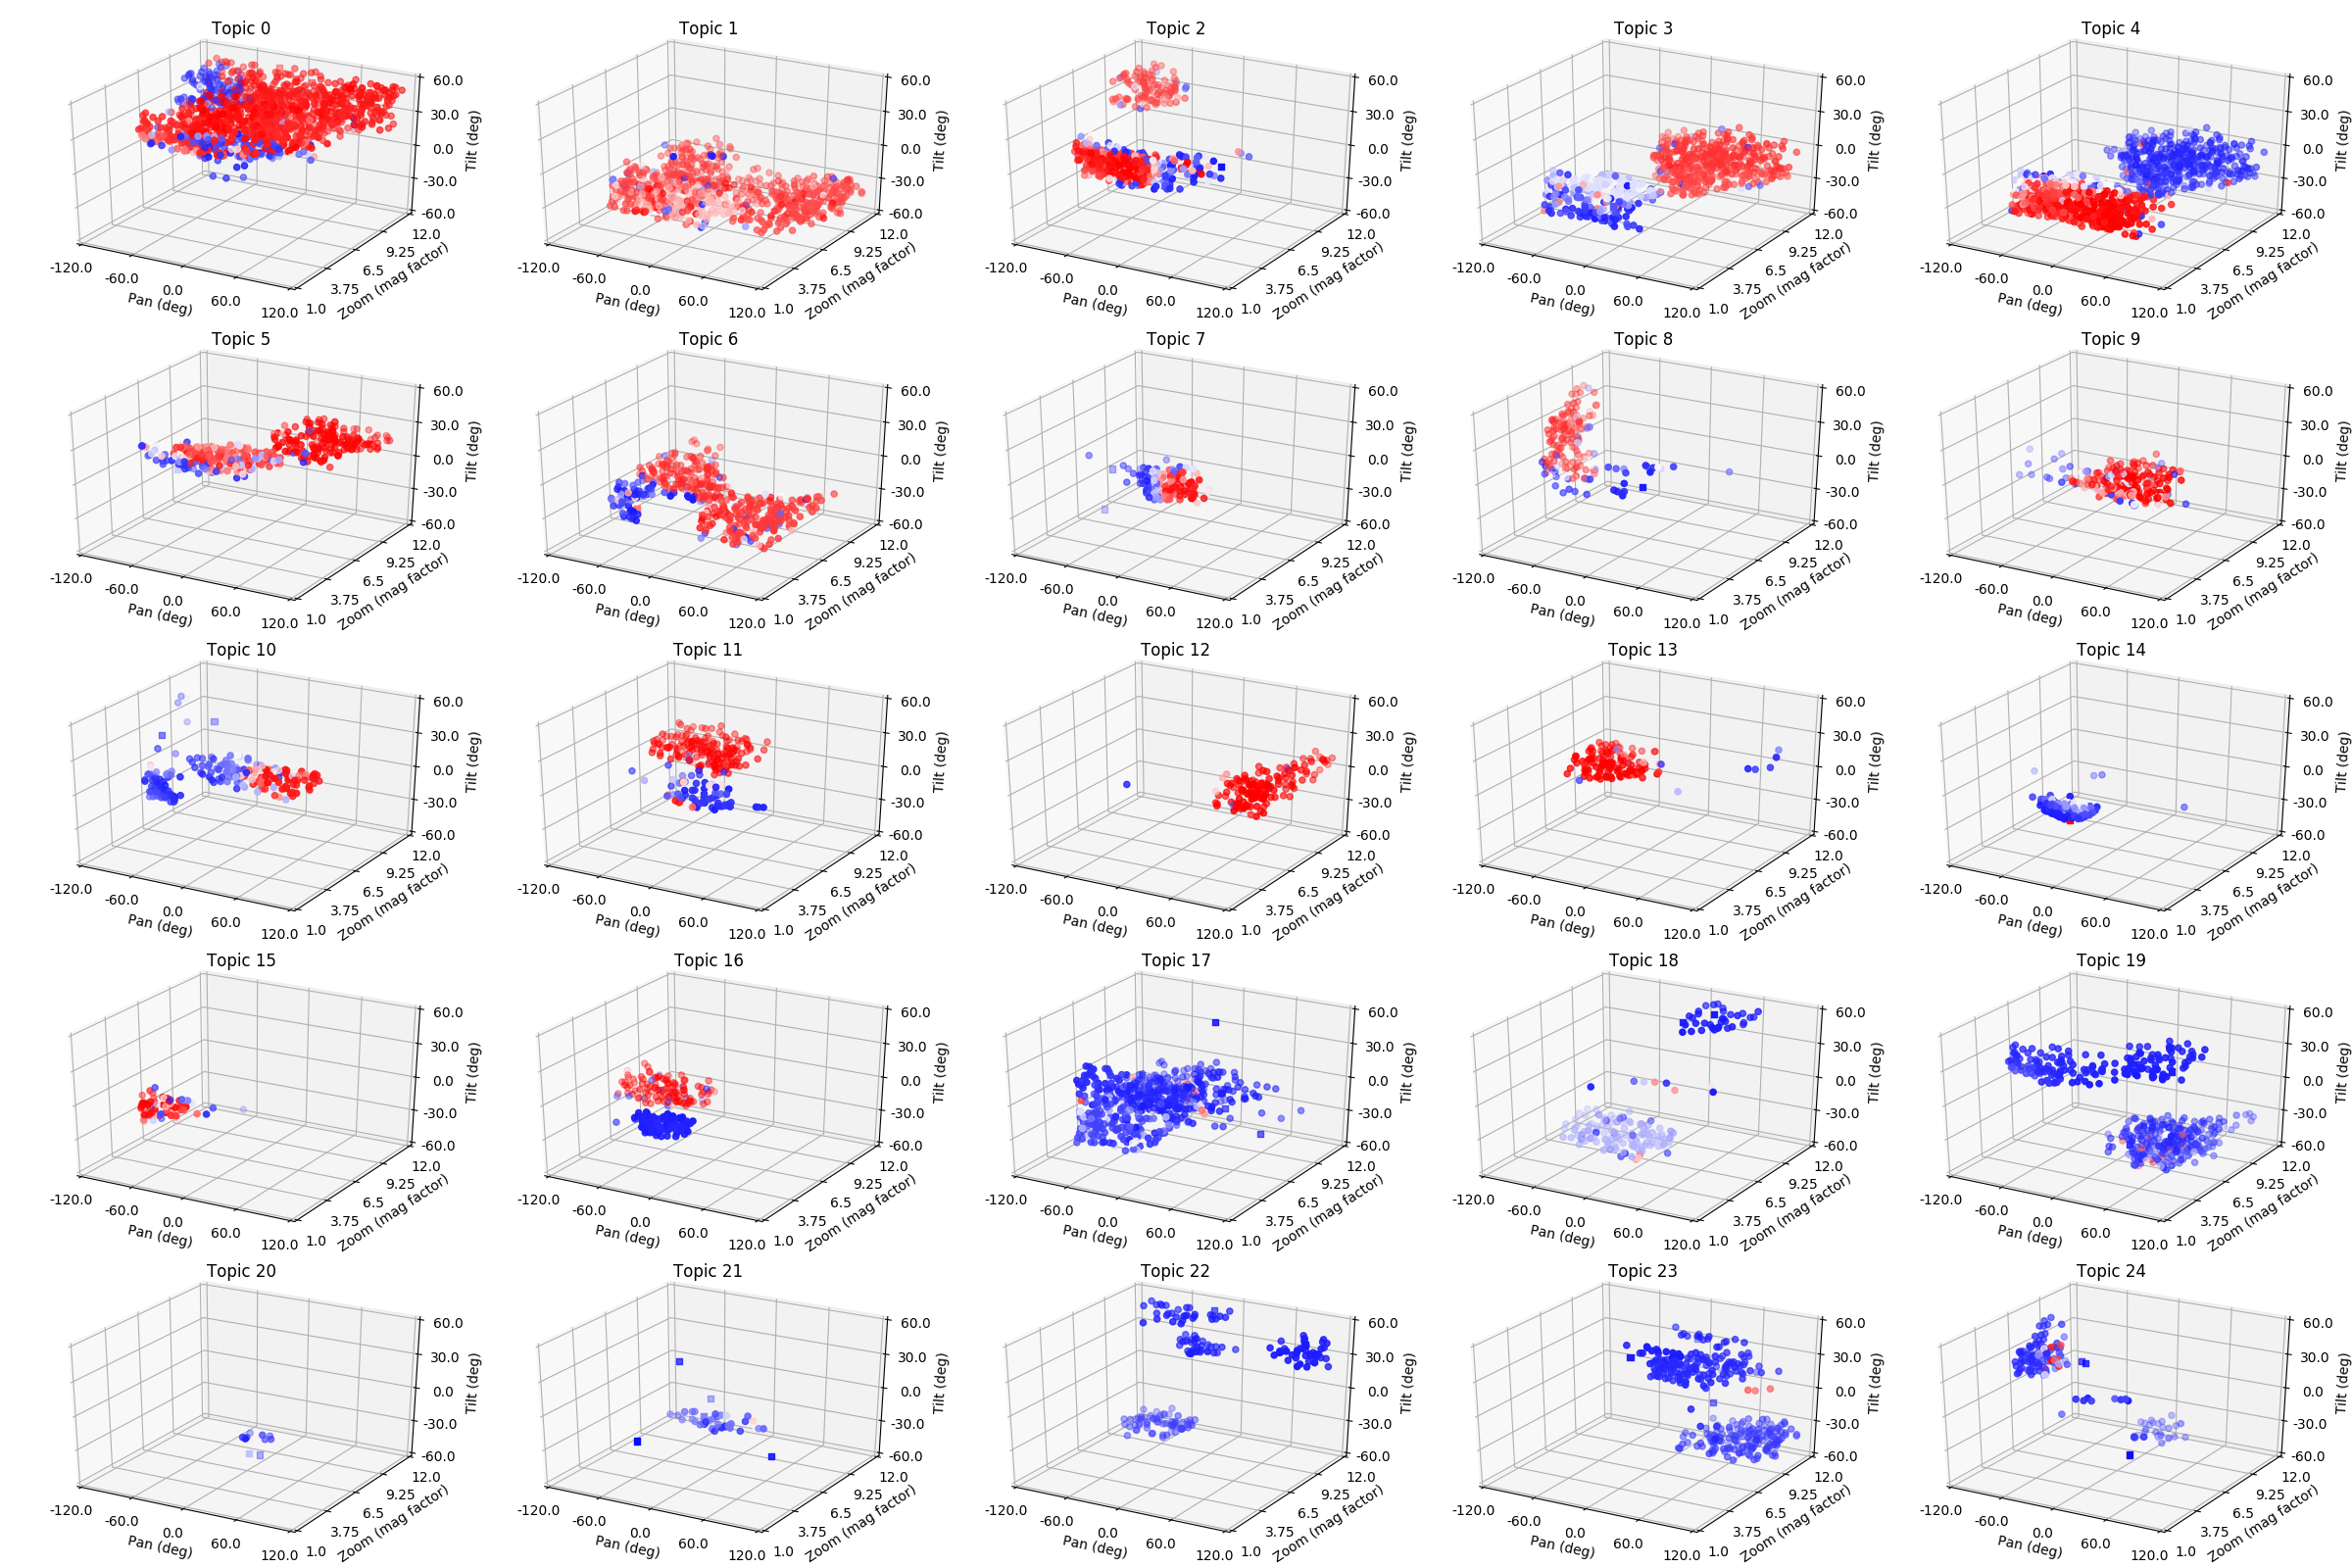
\includegraphics[width=\columnwidth]{figures/ptz/pano_0_map.png}
            \label{fig:pano-0-map}
        } \\
        \subfloat[][]{
            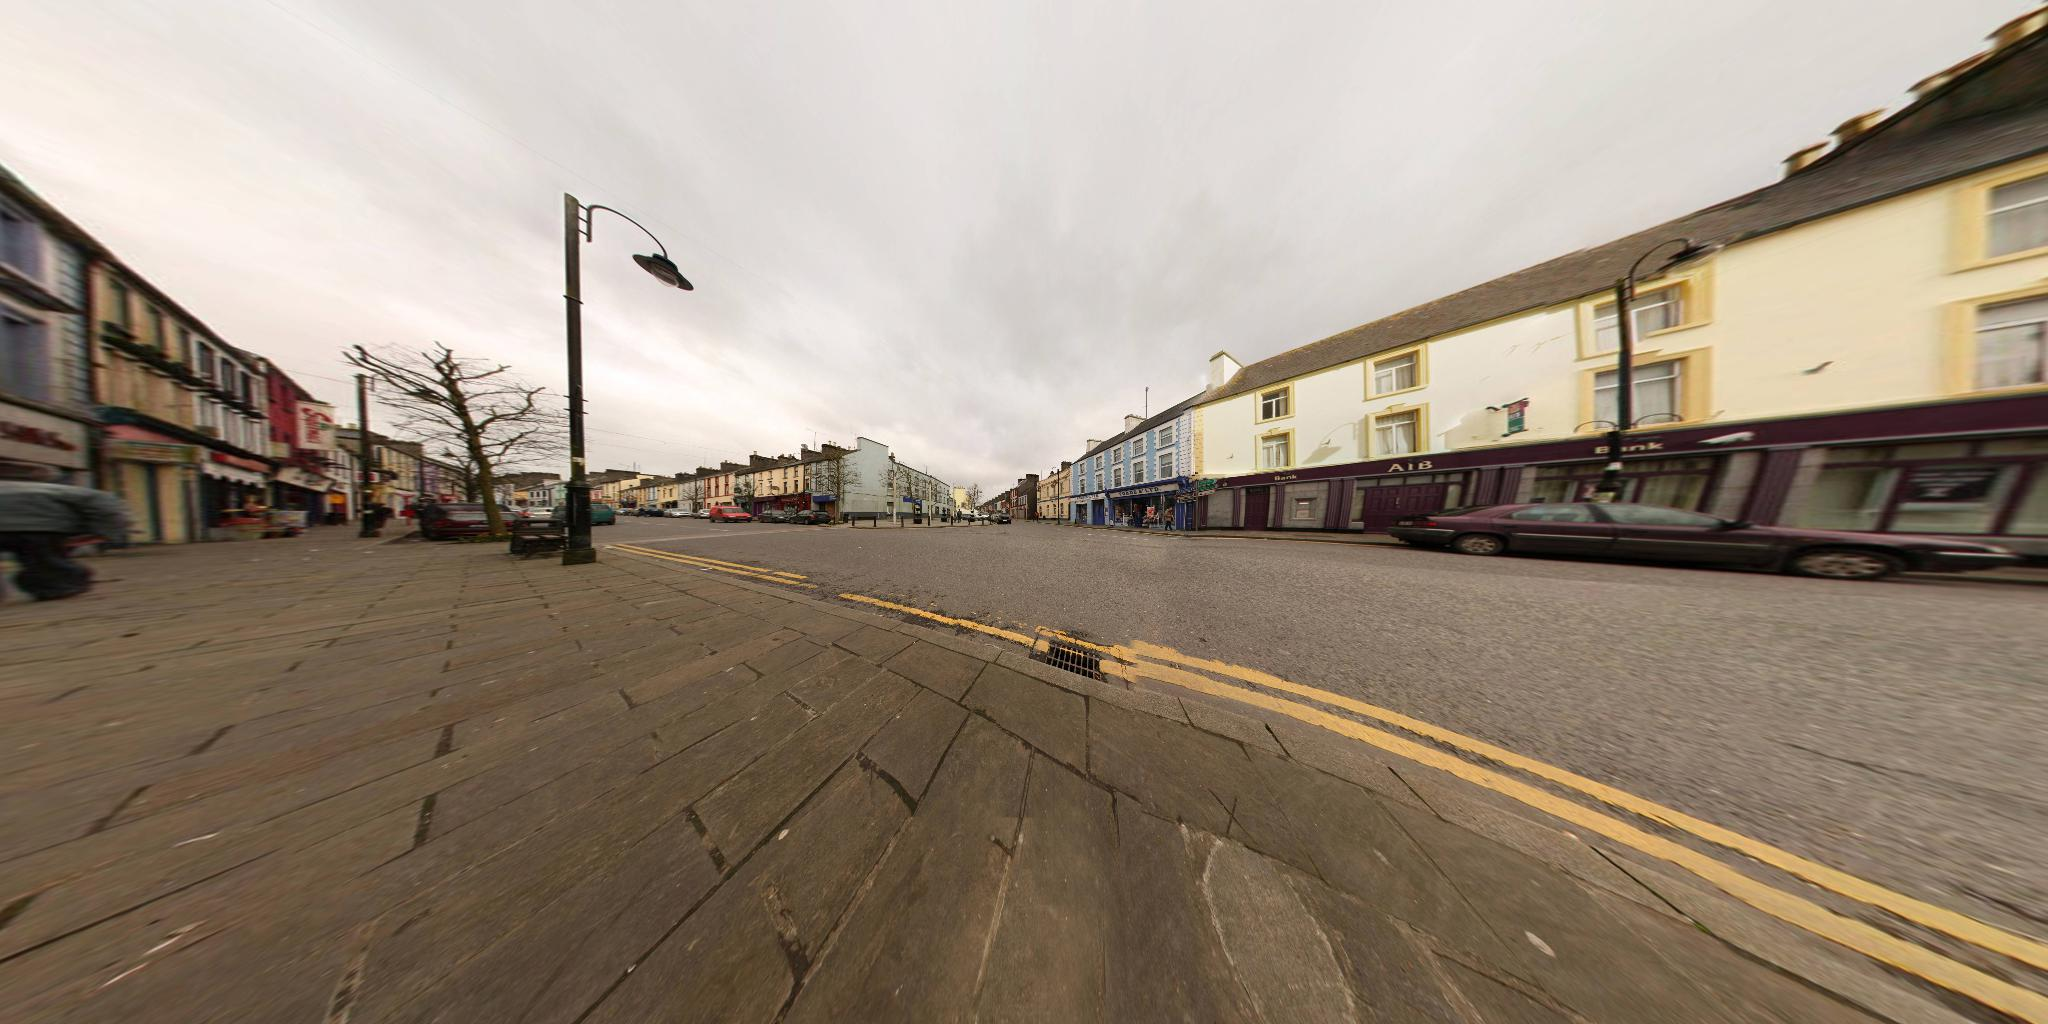
\includegraphics[width=\columnwidth]{figures/ptz/pano_0_pano.jpg}
            \label{fig:pano-0-pano}
        }
    \end{minipage}
    }
    
    \caption{Example spatial prediction model after 50 training observations. \protect\subref{fig:pano-0-pano}} Fish-eye view of the entire panorama \protect\subref{fig:pano-0-topics}, Direct decoding of each topic-distribution ($\Phi_k$), And \protect\subref{fig:pano-0-map} predicted mixture of each topic.
    \label{fig:pano-0}
\end{figure}

\begin{figure}
    \centerline{
    \begin{minipage}{0.6\textwidth}
        \subfloat[][]{
            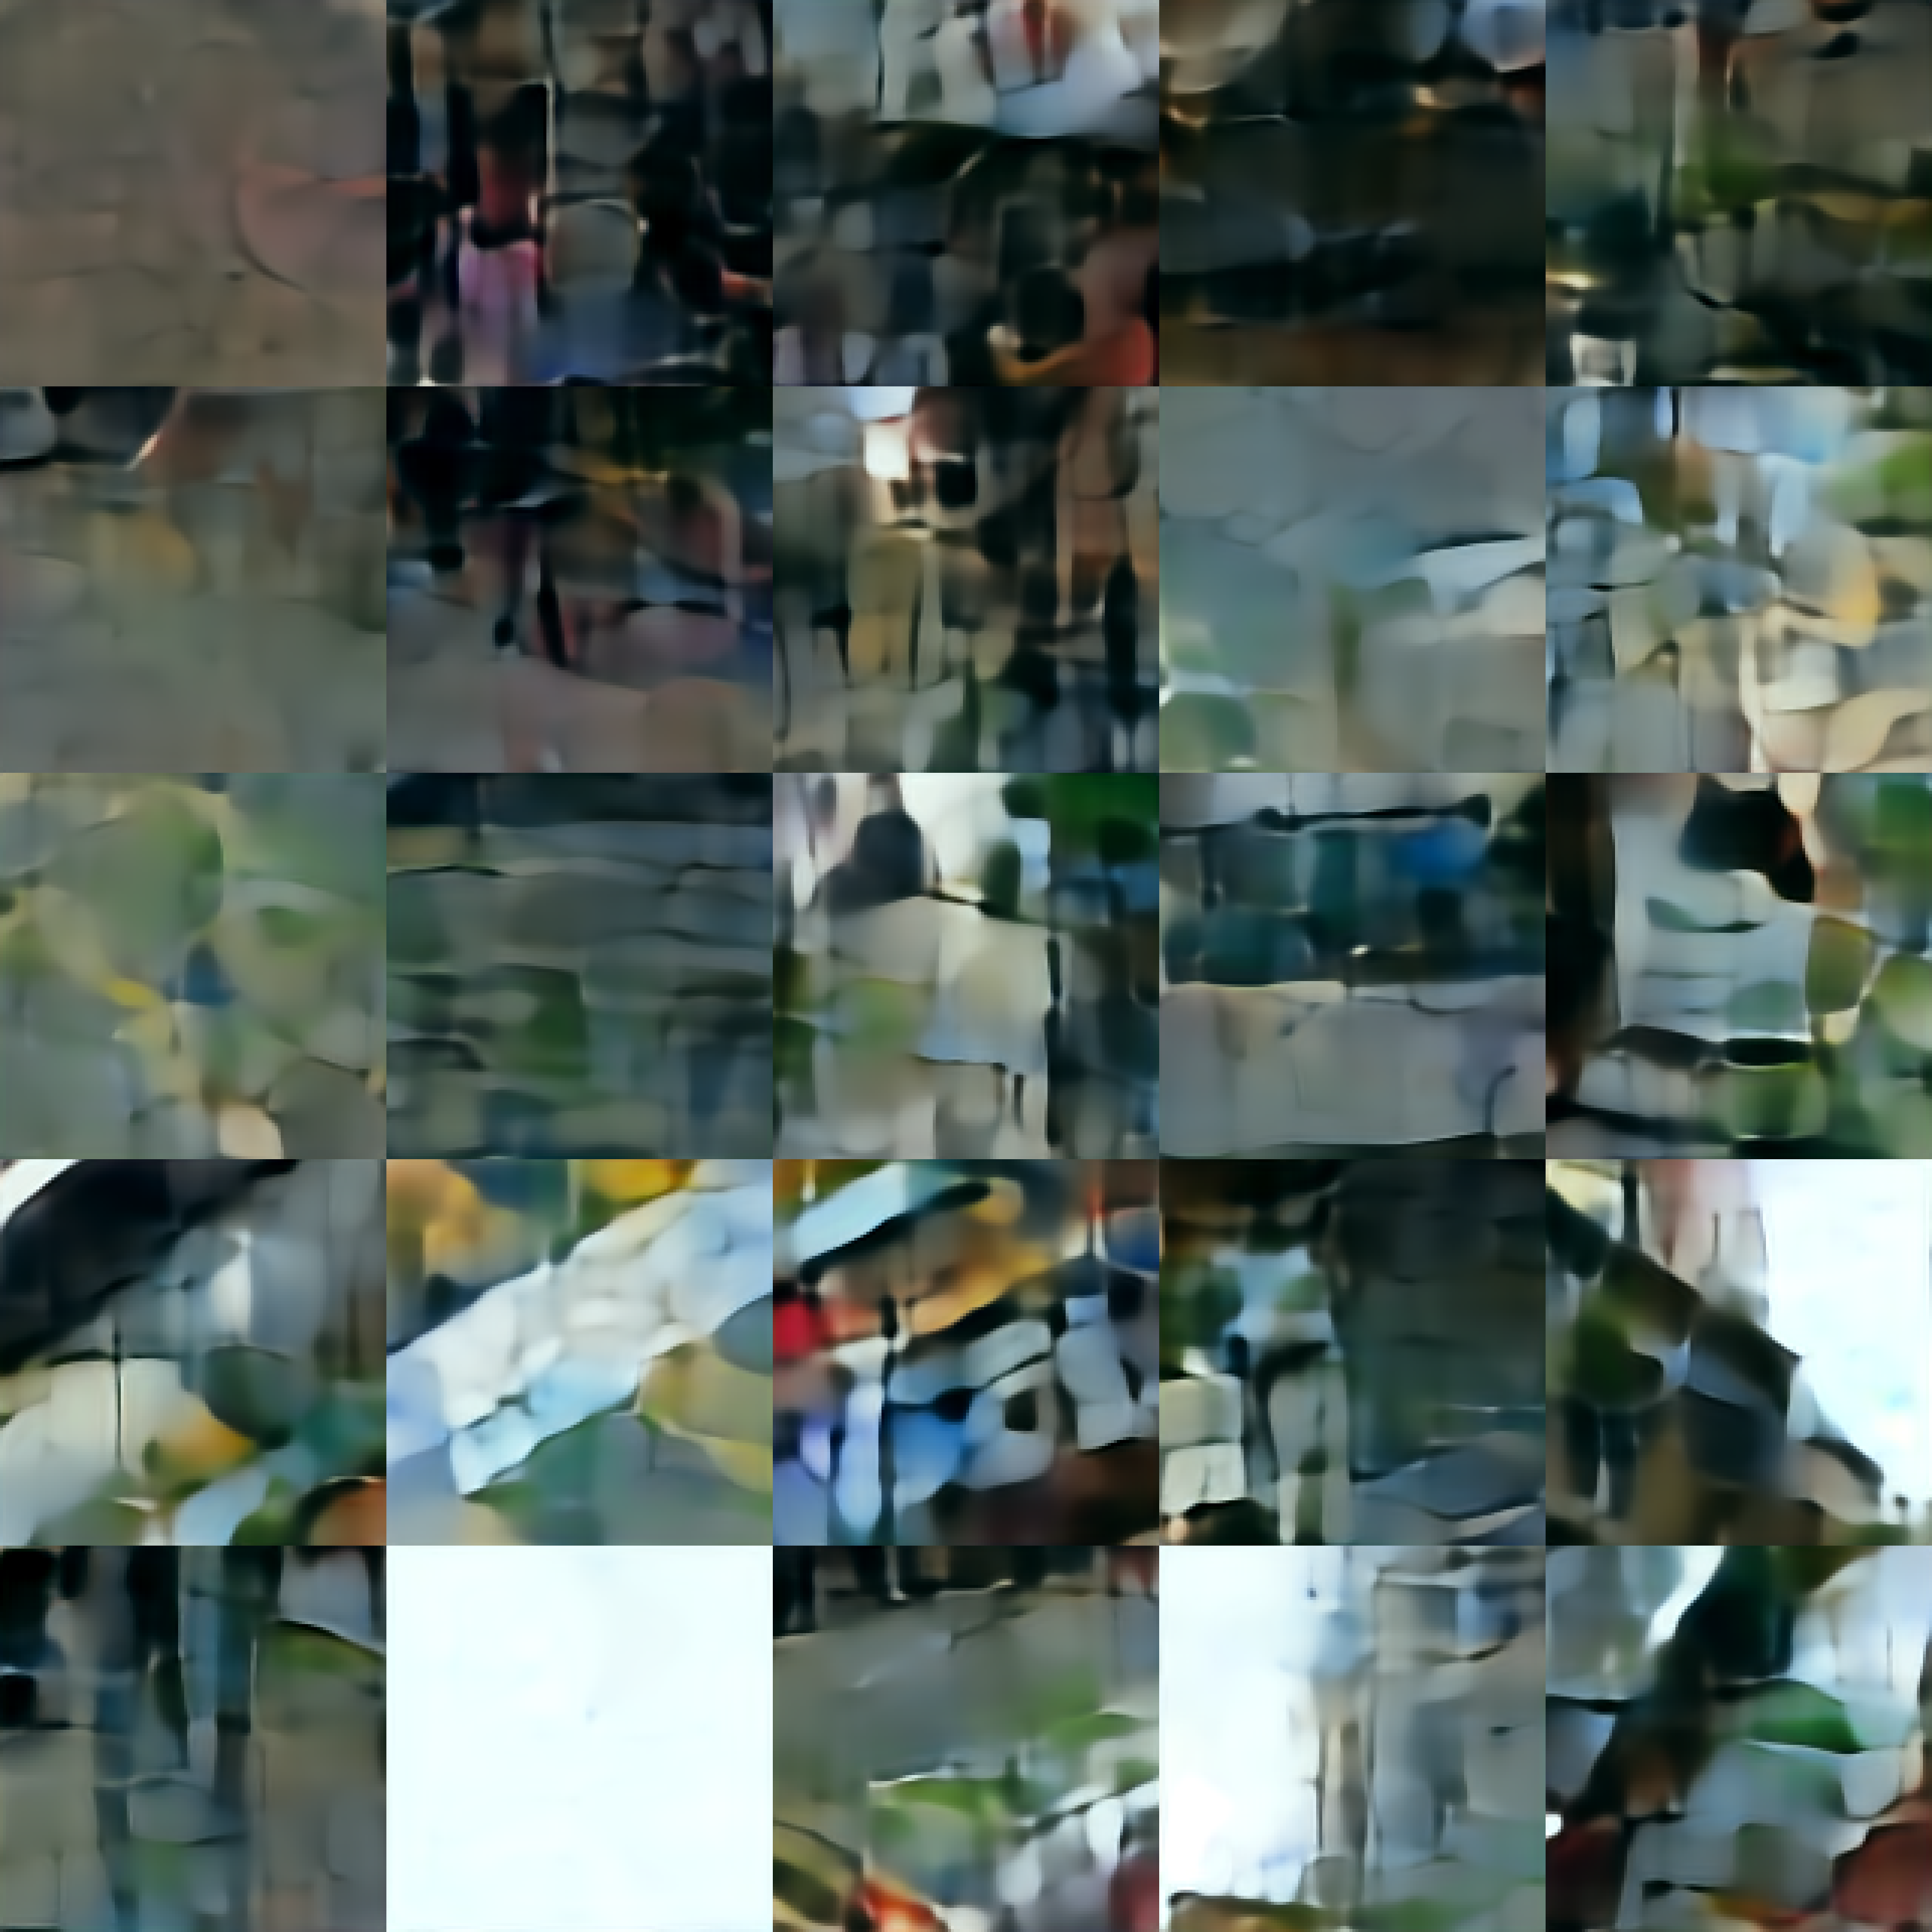
\includegraphics[width=\columnwidth]{figures/ptz/pano_1_topics.png}
            \label{fig:pano-1-topics}
        }
    \end{minipage} \hfill
    \begin{minipage}{0.6\textwidth}
        \subfloat[][]{
            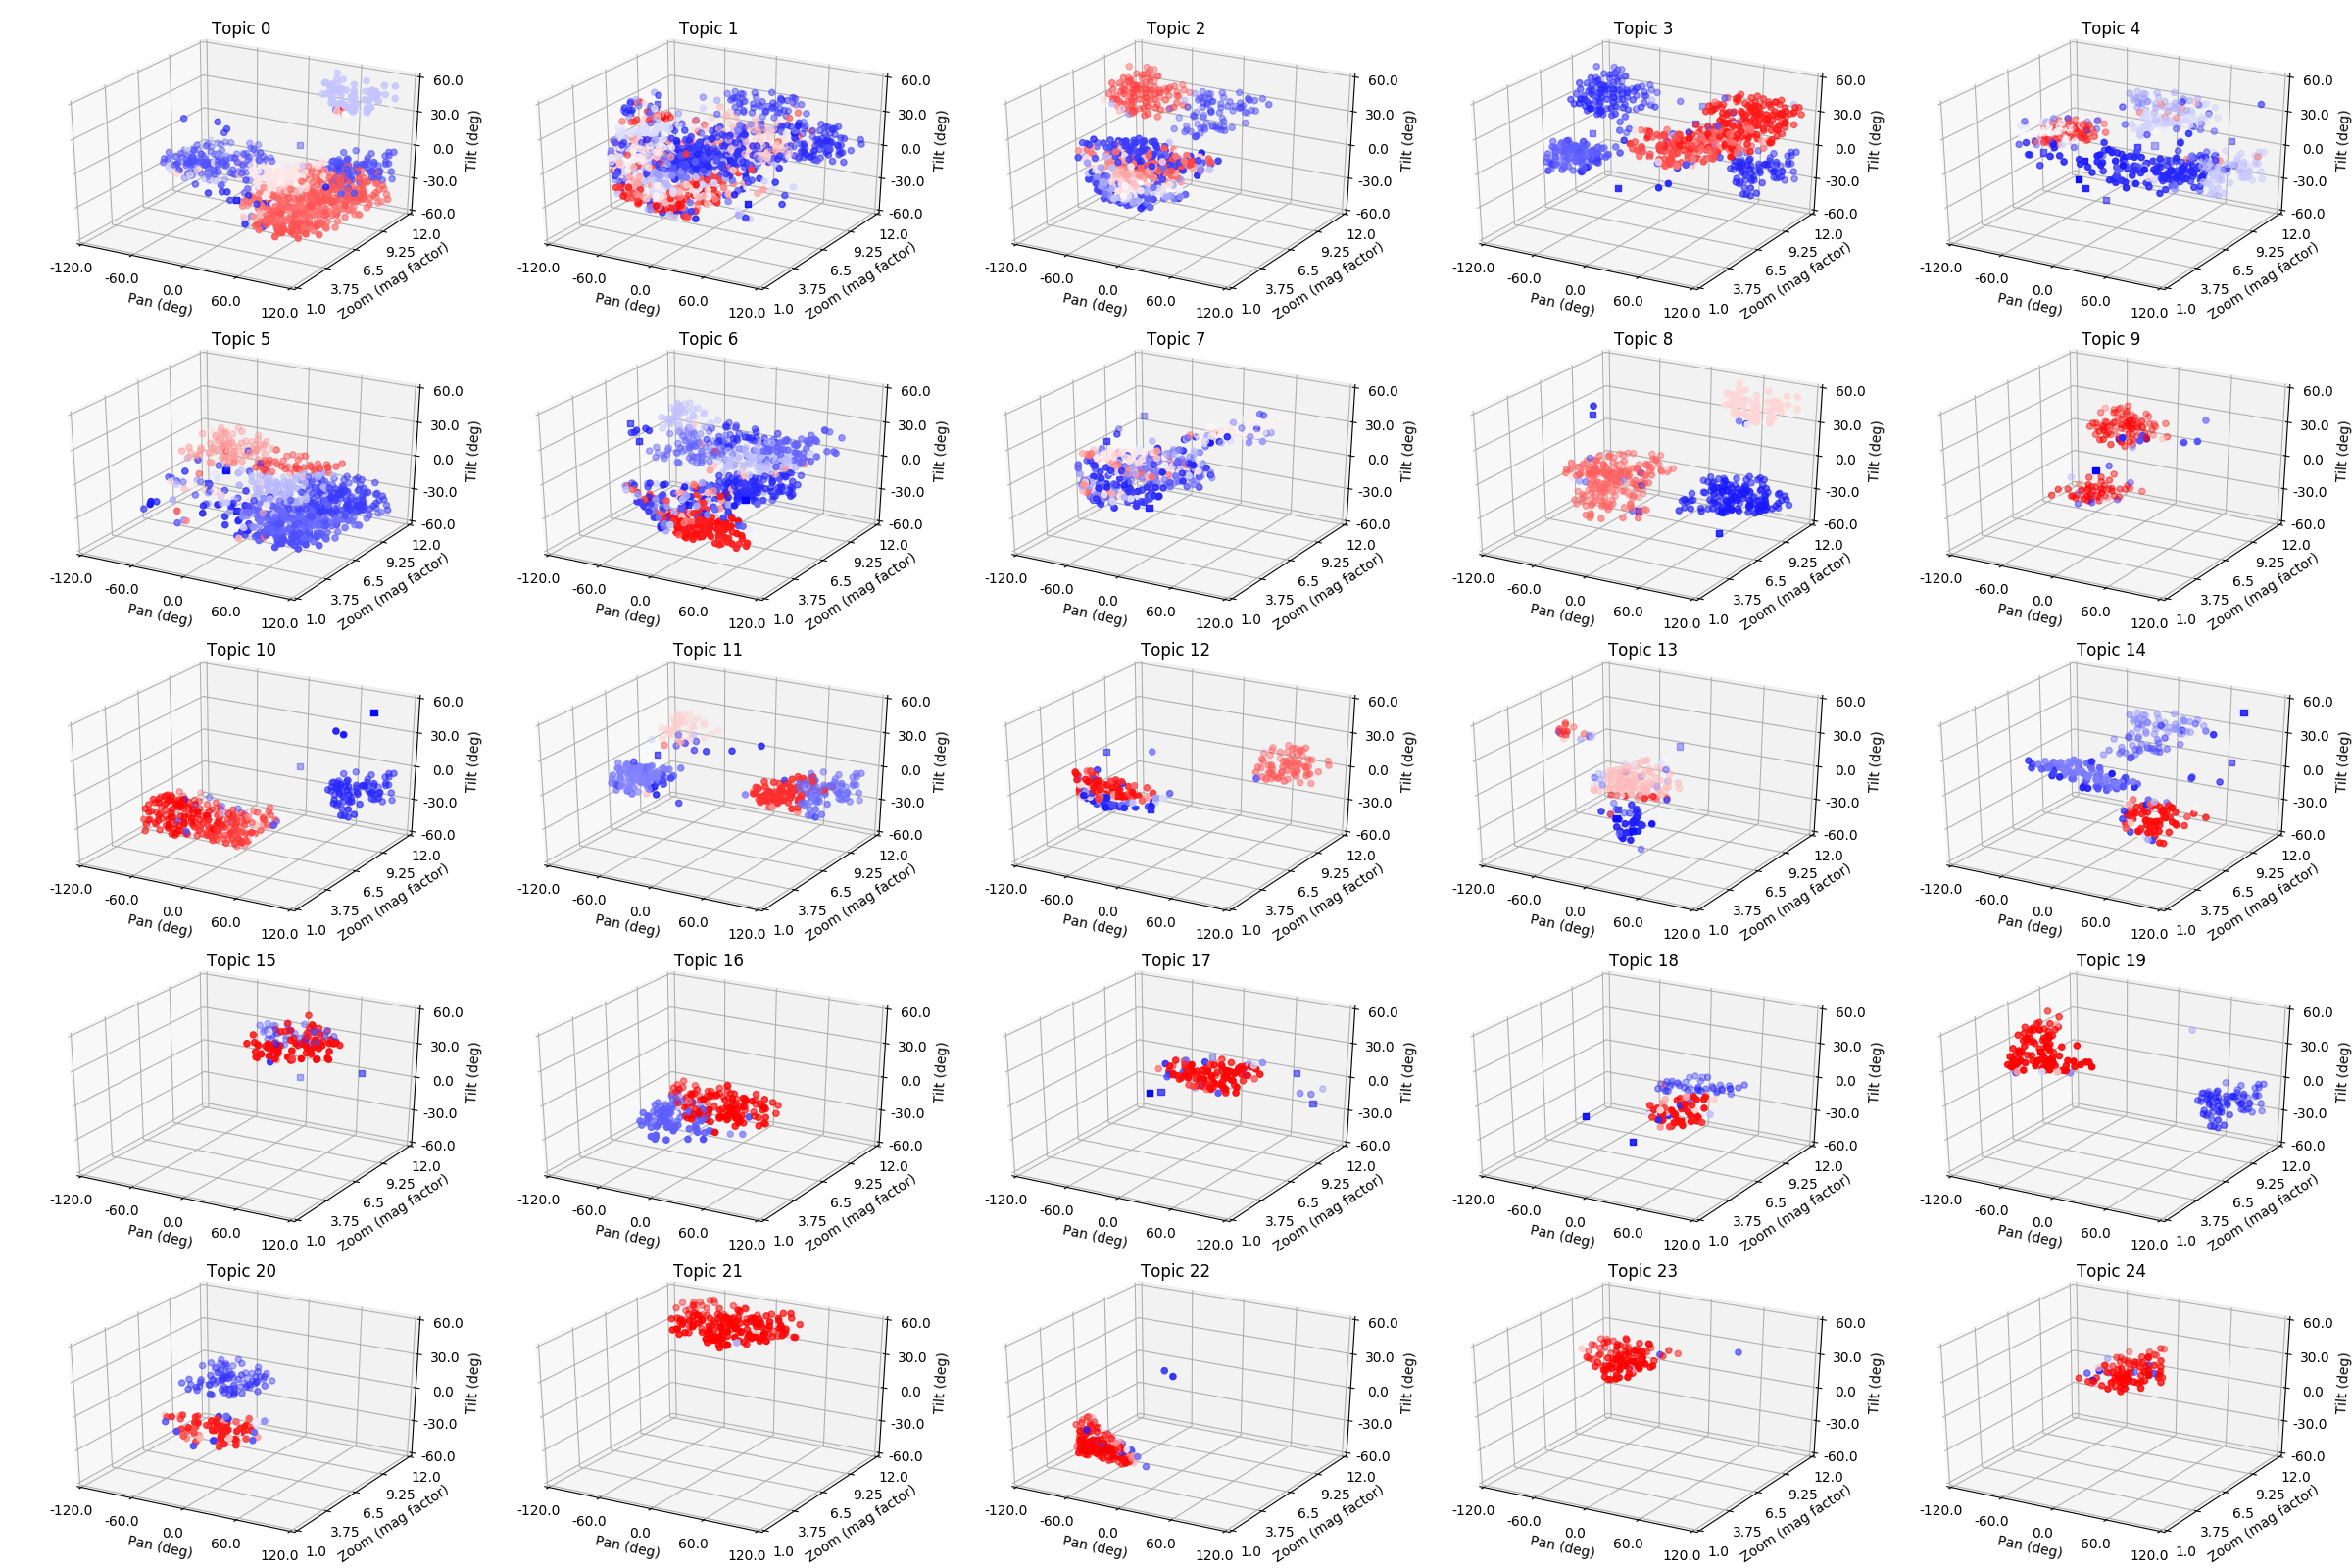
\includegraphics[width=\columnwidth]{figures/ptz/pano_1_map.png}
            \label{fig:pano-1-map}
        } \\
        \subfloat[][]{
            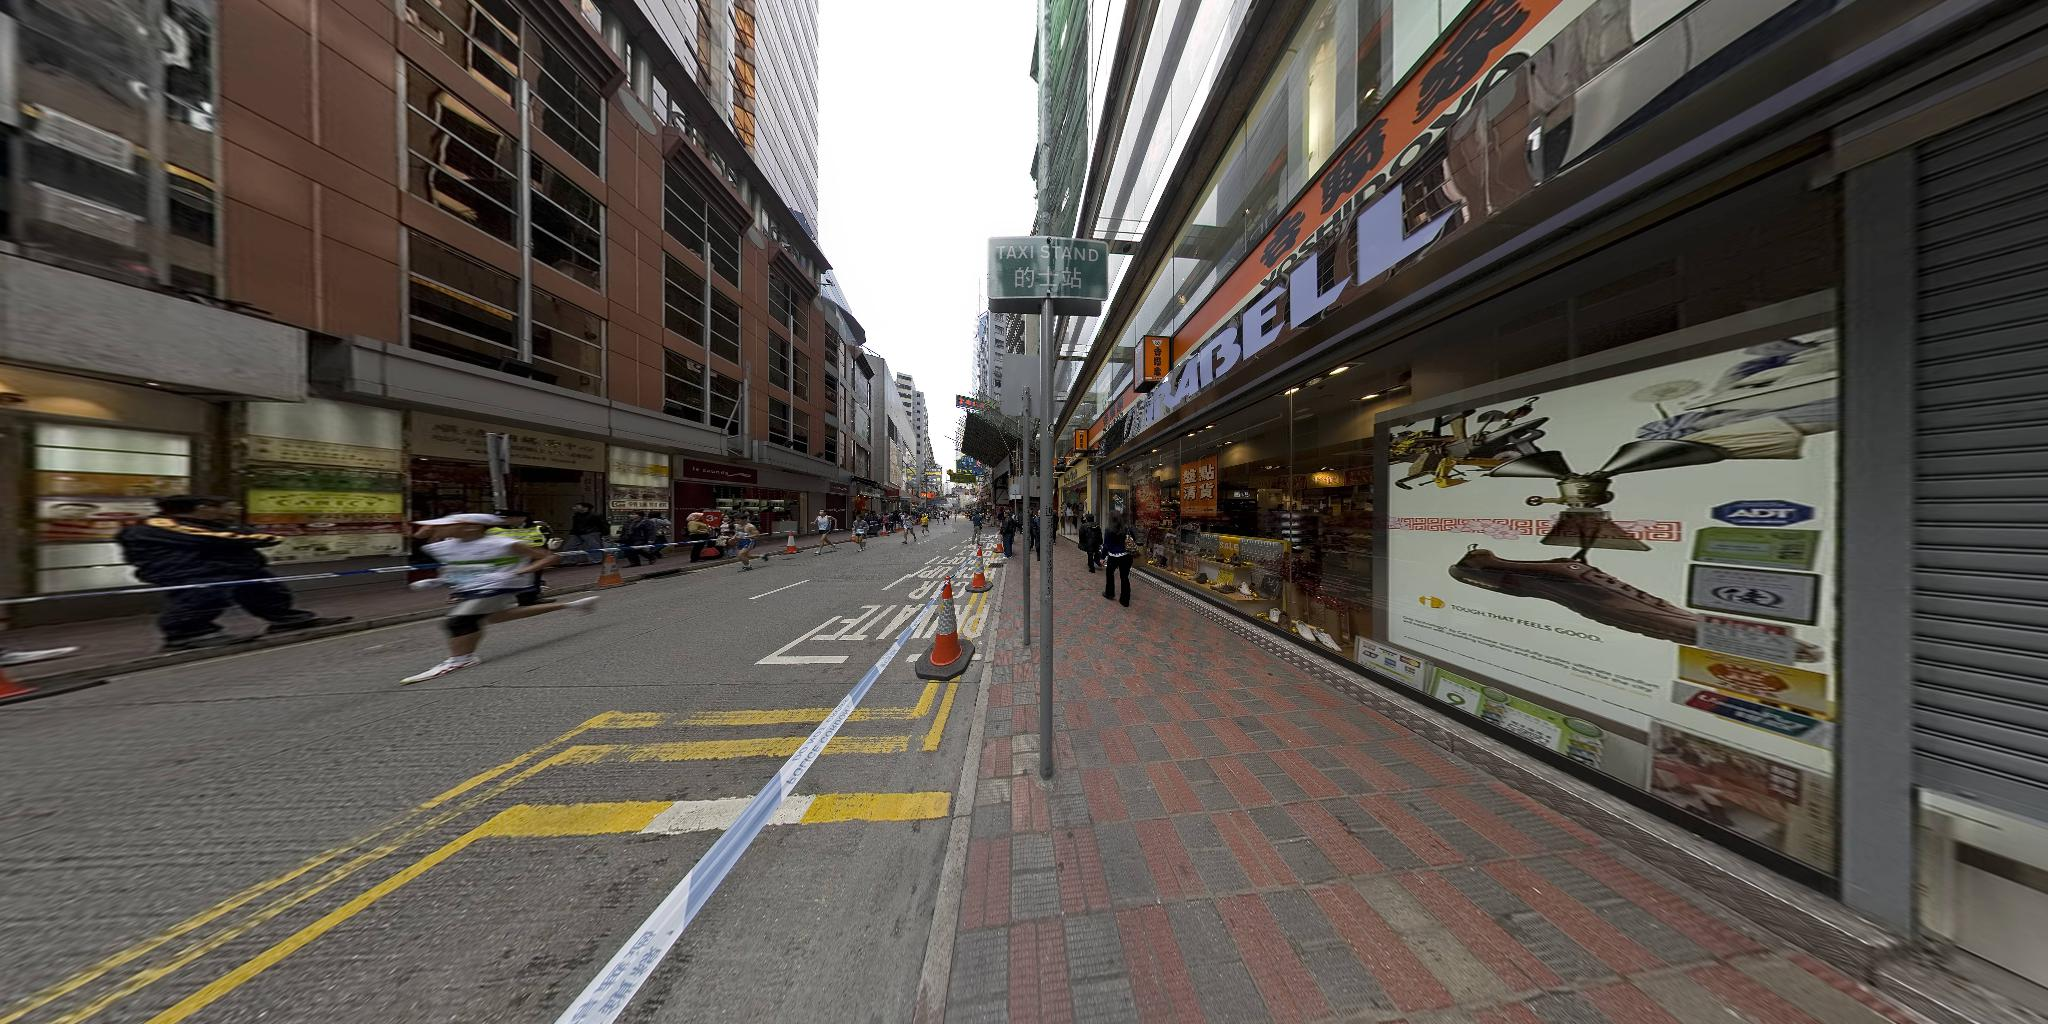
\includegraphics[width=\columnwidth]{figures/ptz/pano_1_pano.jpg}
            \label{fig:pano-1-pano}
        }
    \end{minipage}
    }
    
    \caption{Example spatial prediction model after 50 training observations. \protect\subref{fig:pano-1-pano}} Fish-eye view of the entire panorama \protect\subref{fig:pano-1-topics}, Direct decoding of each topic-distribution ($\Phi_k$), And \protect\subref{fig:pano-1-map} predicted mixture of each topic.
    \label{fig:pano-1}
\end{figure}

\begin{figure}
    \centerline{
    \begin{minipage}{0.6\textwidth}
        \subfloat[][]{
            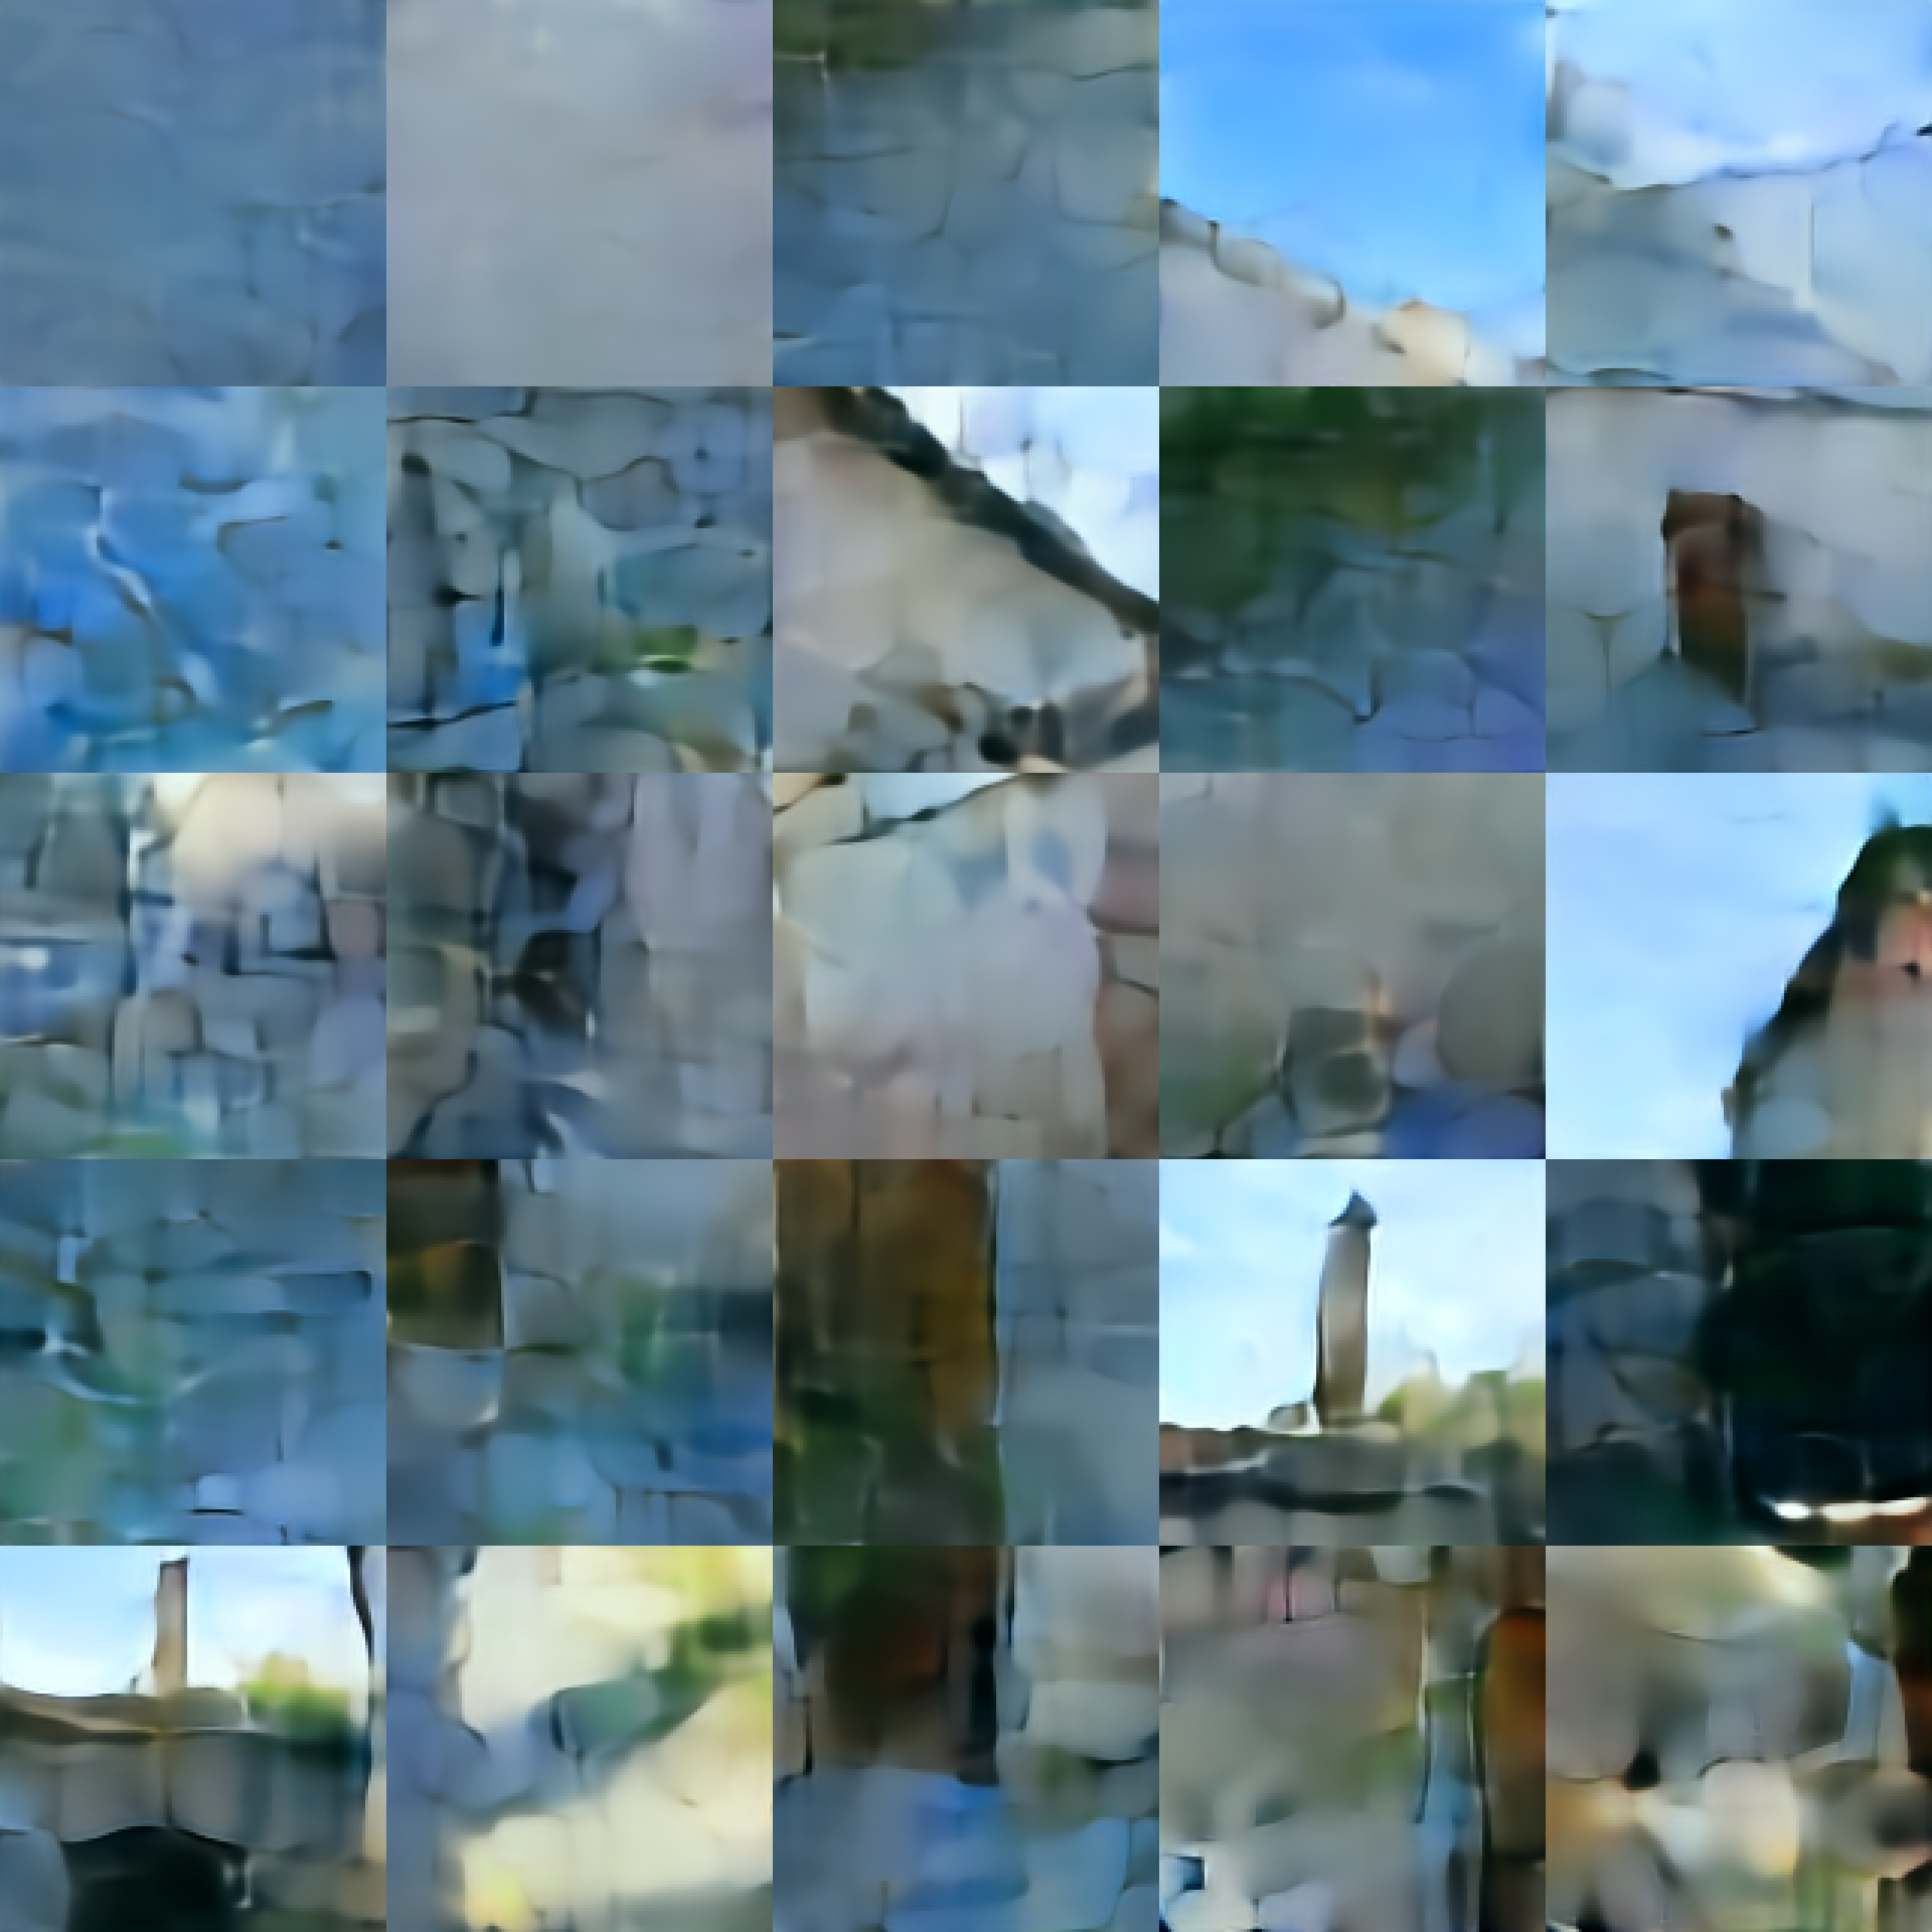
\includegraphics[width=\columnwidth]{figures/ptz/pano_2_topics.png}
            \label{fig:pano-2-topics}
        }
    \end{minipage} \hfill
    \begin{minipage}{0.6\textwidth}
        \subfloat[][]{
            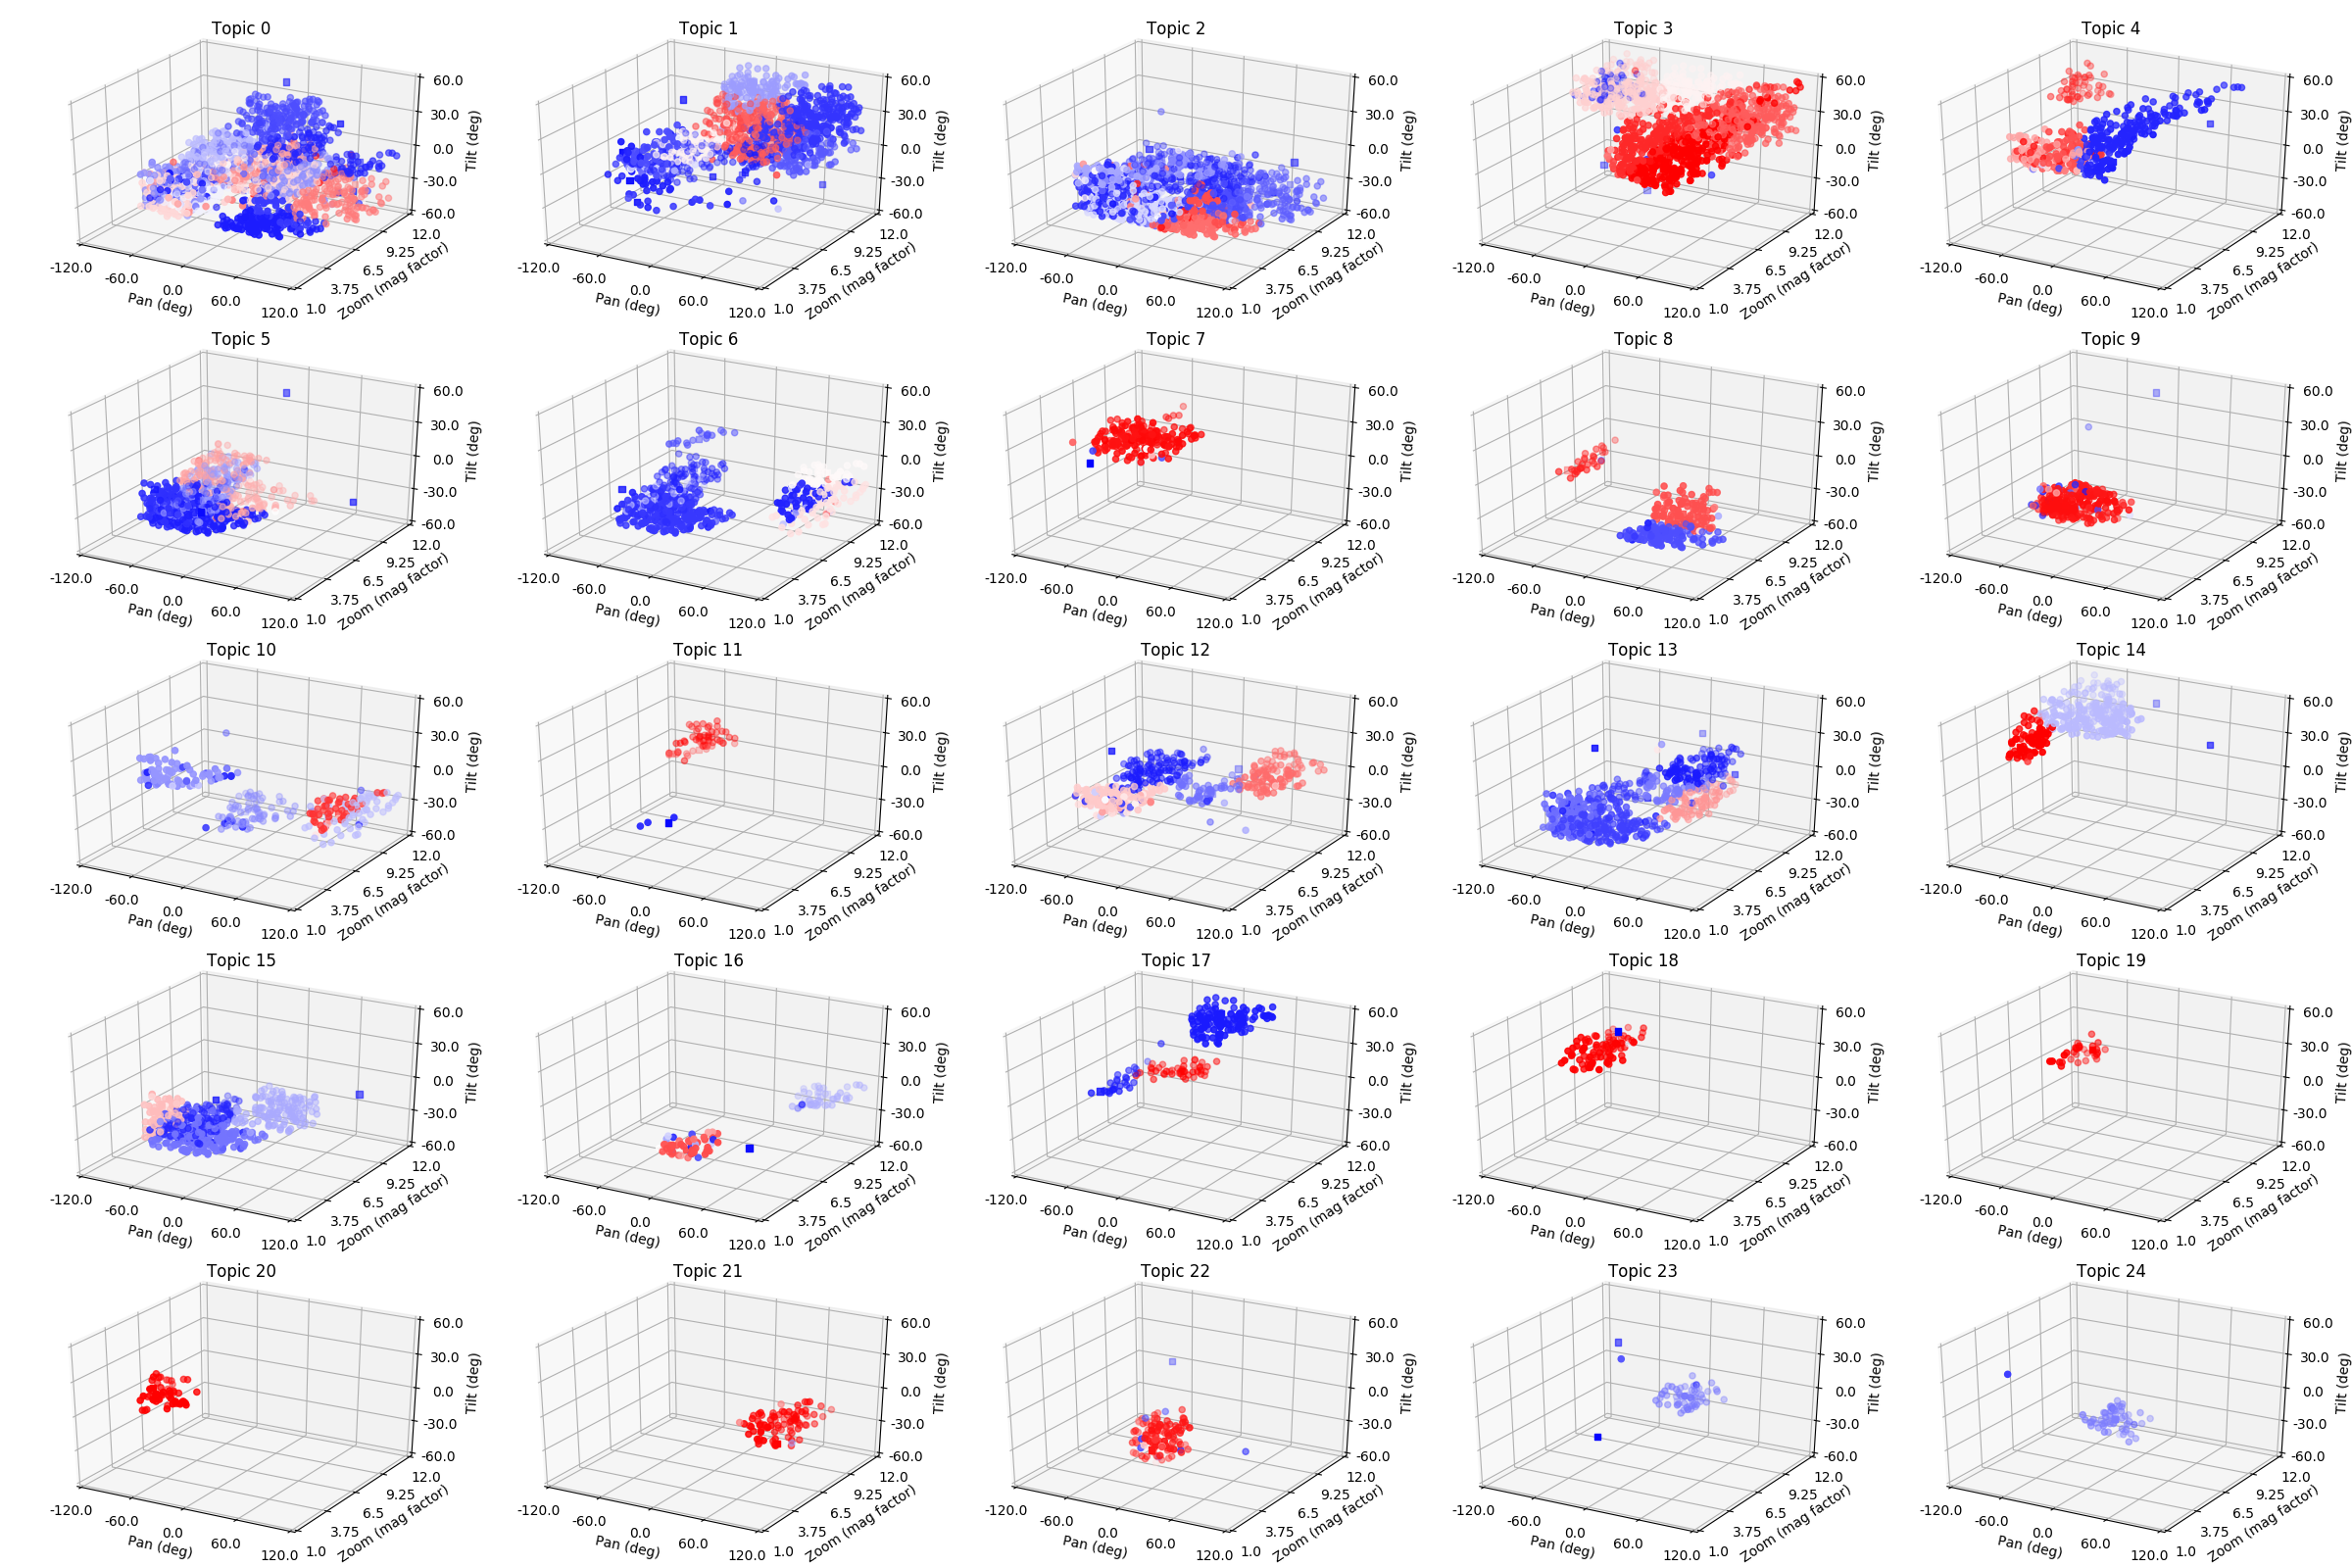
\includegraphics[width=\columnwidth]{figures/ptz/pano_2_map.png}
            \label{fig:pano-2-map}
        } \\
        \subfloat[][]{
            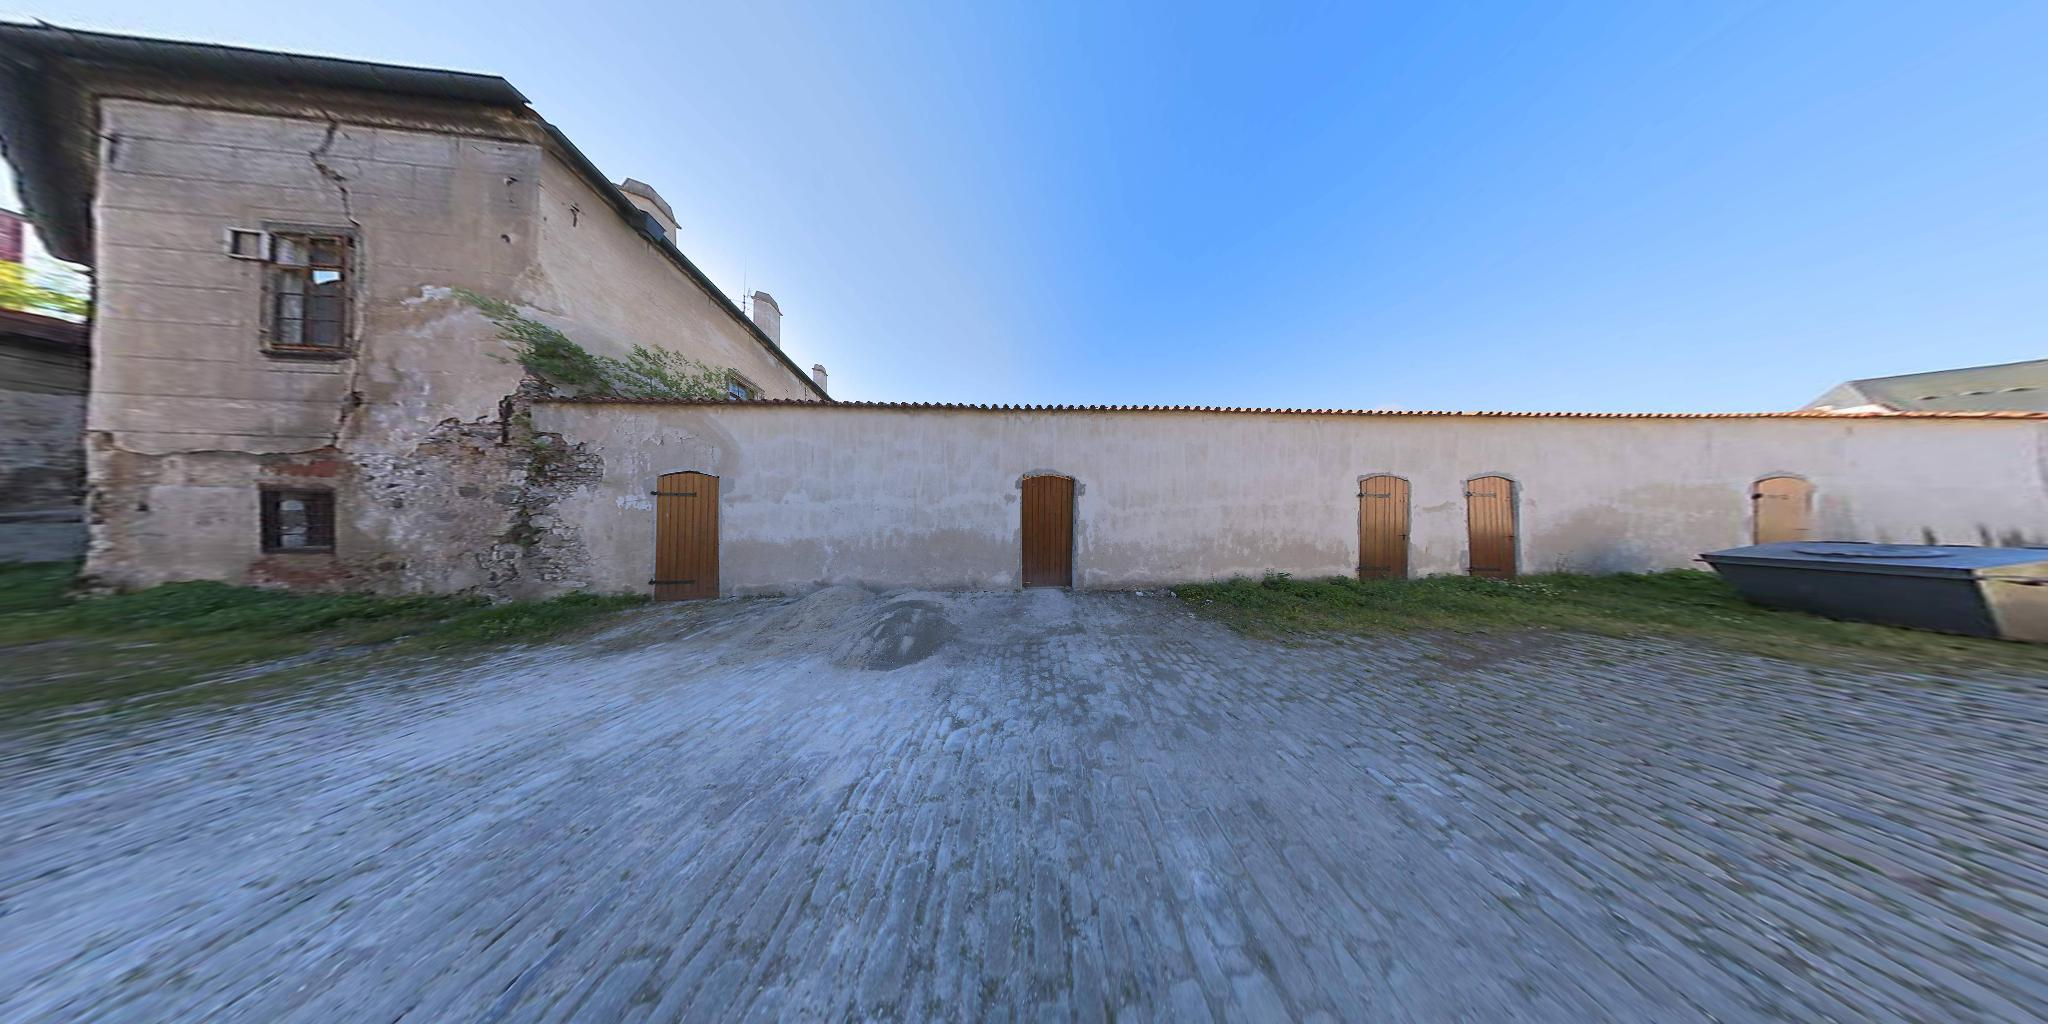
\includegraphics[width=\columnwidth]{figures/ptz/pano_2_pano.jpg}
            \label{fig:pano-2-pano}
        }
    \end{minipage}
    }
    
    \caption{Example spatial prediction model after 50 training observations. \protect\subref{fig:pano-2-pano}} Fish-eye view of the entire panorama \protect\subref{fig:pano-2-topics}, Direct decoding of each topic-distribution ($\Phi_k$), And \protect\subref{fig:pano-2-map} predicted mixture of each topic.
    \label{fig:pano-2}
\end{figure}

In addition to decoding the topic distributions themselves, we can predict the topic prior for a view and the corresponding encoding distribution given the topic distributions, and decode these predicted encodings. We evaluate our system based on the root mean squared error (RMSE) pixel value between the predicted images and the true image at that view. We call views that where we have run topic inference and topic map training but not topic refinement `observed'. At observed views our model predicts exactly the topic prior observed in that location, and so is able to represent the information encoded in the topic model without external loss.

As performance baselines, we trained two additional autoencoders with similarly constrained latent spaces offline, on the SUN360/street training set used to train the CIB-AE. First, we trained a plain CAE, without a categorical distribution latent space or additional loss terms beyond the MSE. We copy the architecture of the CIB-AE up to the softmax layer, and then add 3 additional fully connected layers of sizes 4096, 2048, and 1024, with ReLU and BatchNorm nonlinearities and with a final latent representation of 25 dimensions to complete the encoder. As with CIB-AE, the decoder is symmetric with the encoder. We initialilzed the weights of the encoder by copying them from the pretrained CIB-AE where possible, and trained the CAE using the same procedure as the CIB-AE.

In addition, we trained the previously discussed vector-quantized variational autoencoder (VQ-VAE, \citep{vqvae2017}) with a codebook of size $25 \times 8192$, identical to the size of the topic model's $\Phi$ parameter. VQ-VAE is a state of the art autoencoder model designed to address many of the same issues as the topic model. However it cannot be trained online like the topic model, and so it must fit a globally salient representation into the fully compressed $25$-dimensional encoding sapce. We found that VQ-VAEs are very sensitive to architecture choices. For a fair comparison, it would be preferrable to use a VQ-VAE with spatial resolution $4 \times 4$ and feature size $512$ for each spatial block, however we could not escape posterior collapse using this representation. In fact, the only spatial resolution we found that attained reasonable results was the one the original authors demonstrated, therefore our comparisons are against a VQ-VAE with spatial resolution $32 \times 32$ and a feature size of just $8$ for each spatial block.

For the baseline approaches, we apply a similar energy-based prediction model as for the topic-priors, however as the encodings are not probability distributions, we mix them by performing the weighted sum directly rather than in log-probability space. In addition, the cross-validation metric for $w$ is the MSE of the predicted encodings rather than $D_{JS}$. Note that the baselines are not trained with spatial information, so we would not expect this method to achieve the same performance as with the spatially smooth topic model.

Fig.~\ref{fig:encoding-obs-strip} shows examples of the autoencoding performance of the various systems through their 25 dimensional representations. The leftmost column is the observed image and the second column is the CIB-AE autoencoding of that image. The subsequent columns are the decoded neighborhood-word distribution, the VQ-VAE autoencoding, and the CAE autoencoding. The CAE is not able to capture any detail in this regime, the gray images seen are characteristic of the encoder collapse problem mentioned previously. The VQ-VAE, unsurprisingly because of its high-spatial resolution and low feature dimensionality, captures the spatial structure of the image relatively well, but loses much of the color and distorts the texture. Finally, our approach is competetive with the VQ-VAE, featuring images that are more spatially distorted, but interestingly, that enhance the color contrast of its input images. Fig.~\ref{fig:encoding-pred-strip} is similar, however it shows unobserved views, predicted through the topic prediction model.

\begin{figure}
    \begin{center}
    \subfloat[]{
        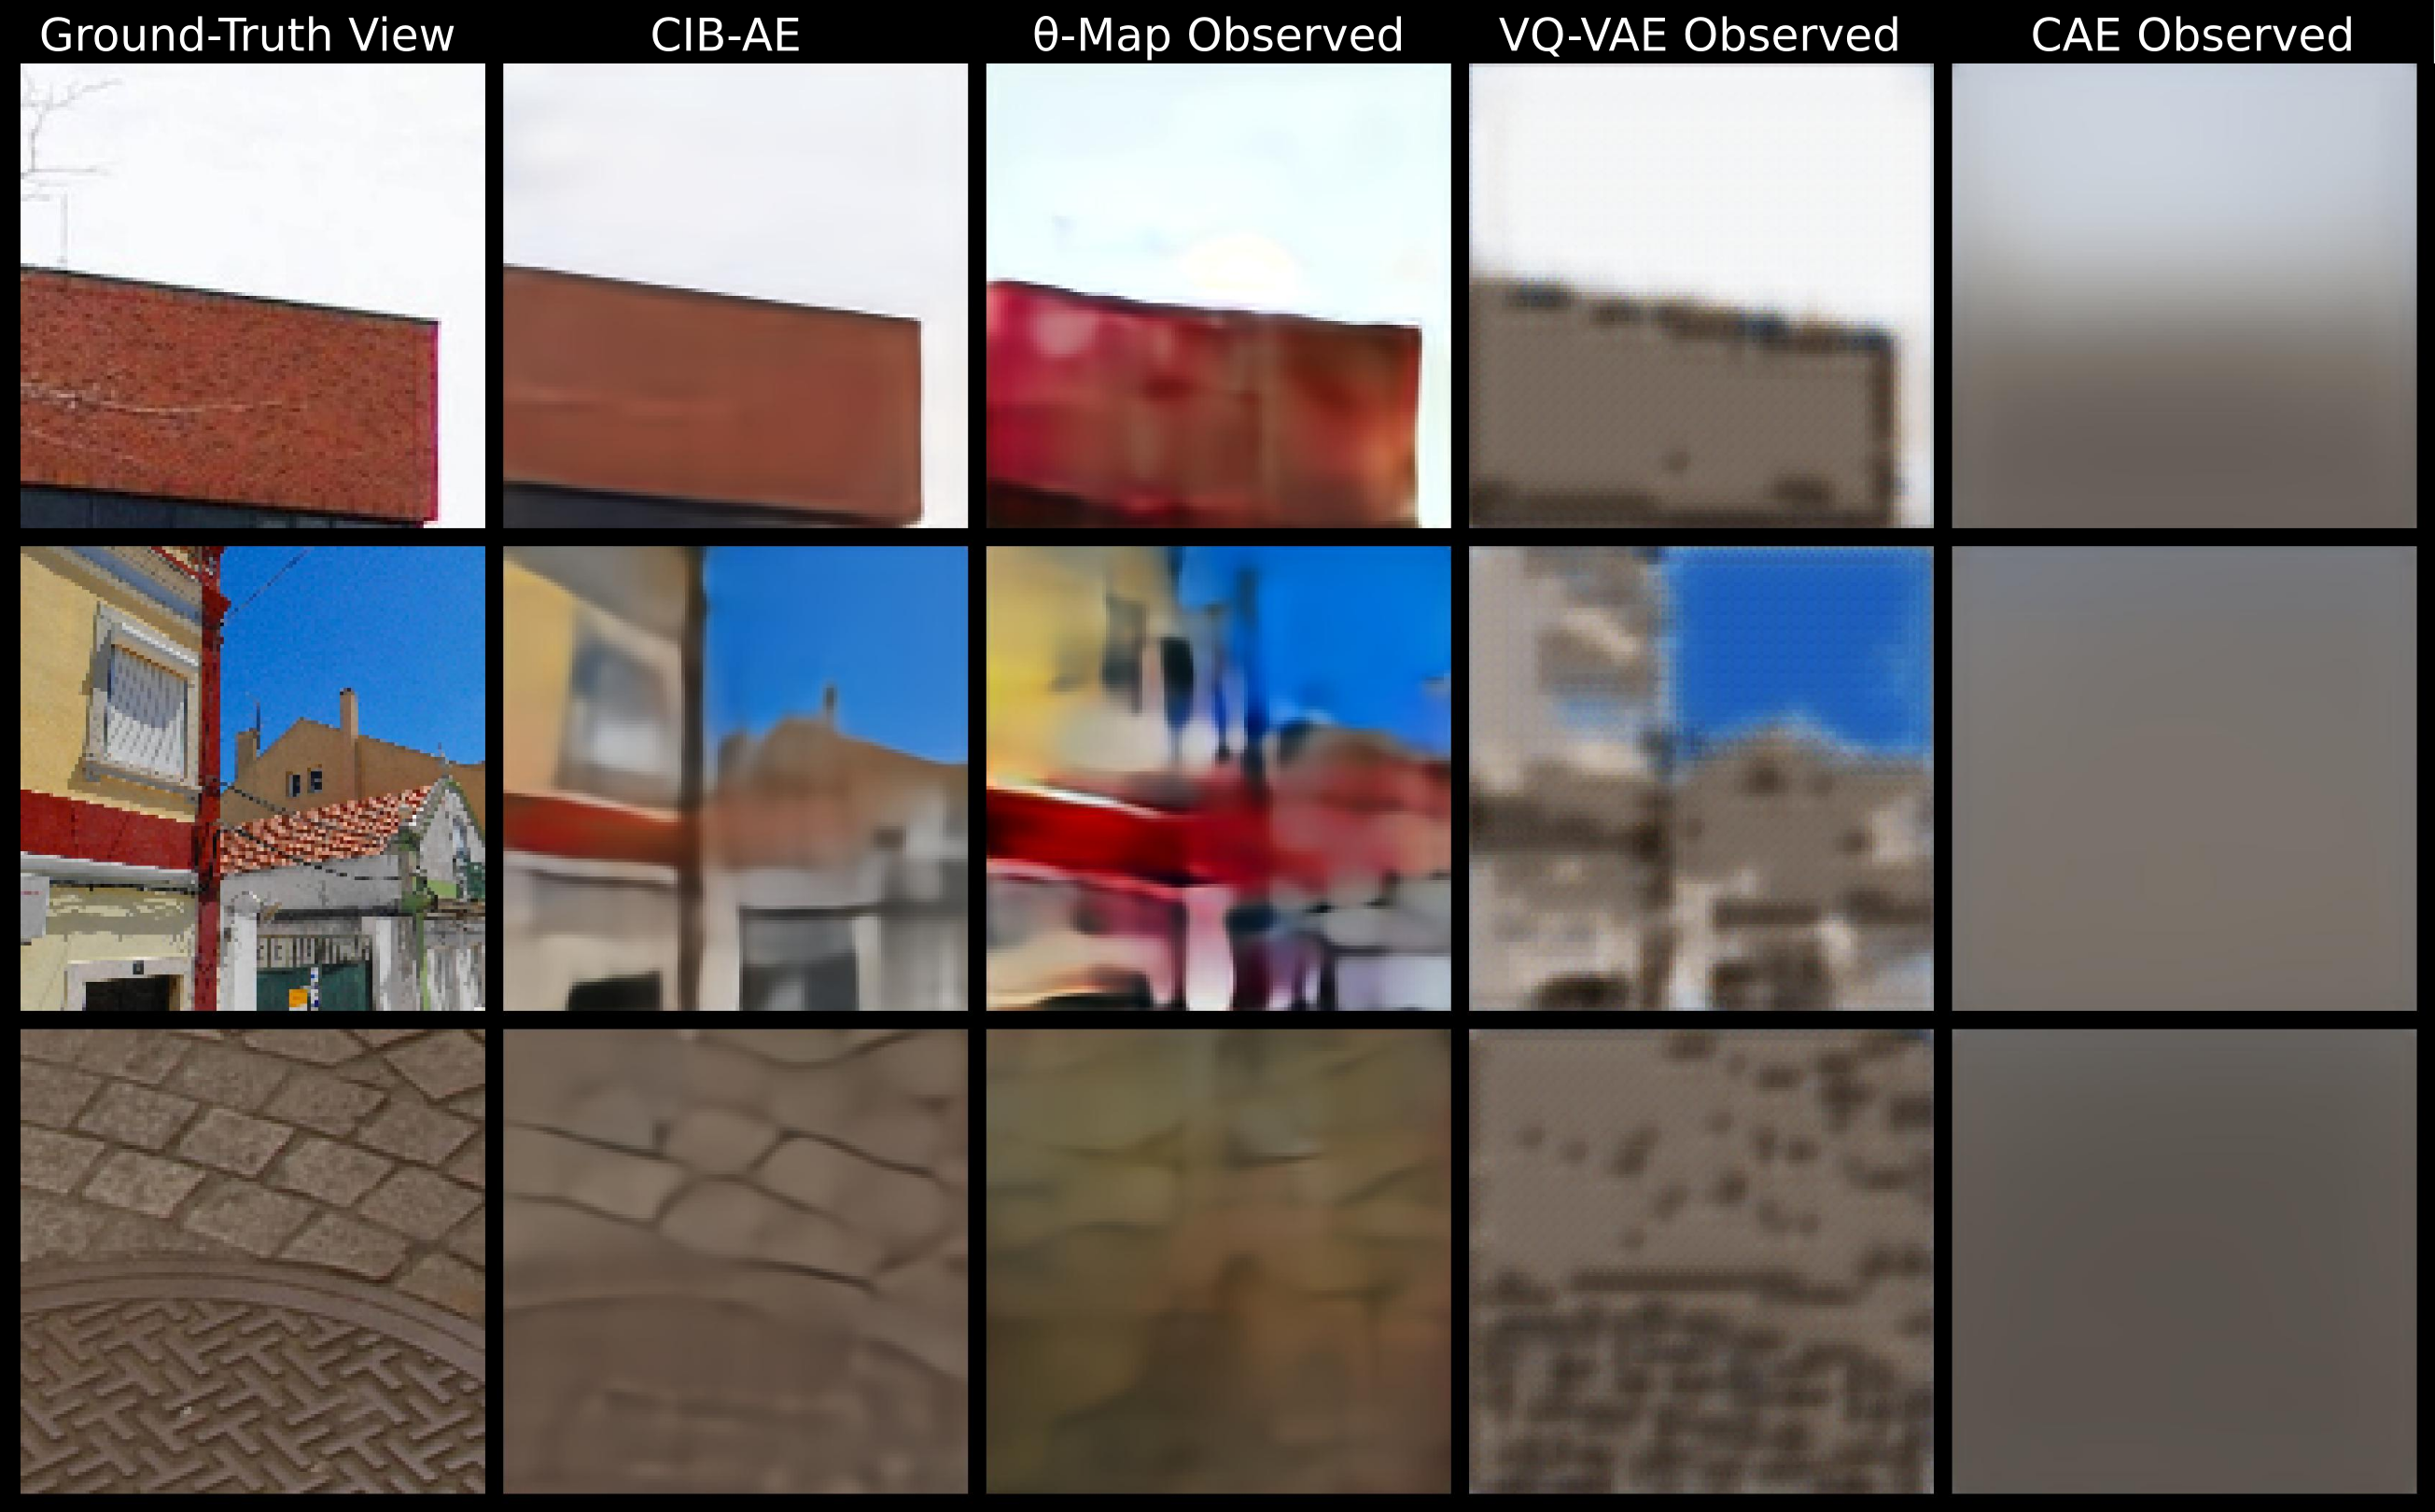
\includegraphics[width=0.89\columnwidth]{figures/ptz/train_stacked_intext.png}
        \label{fig:encoding-obs-strip}
    }\\
    \subfloat[]{
        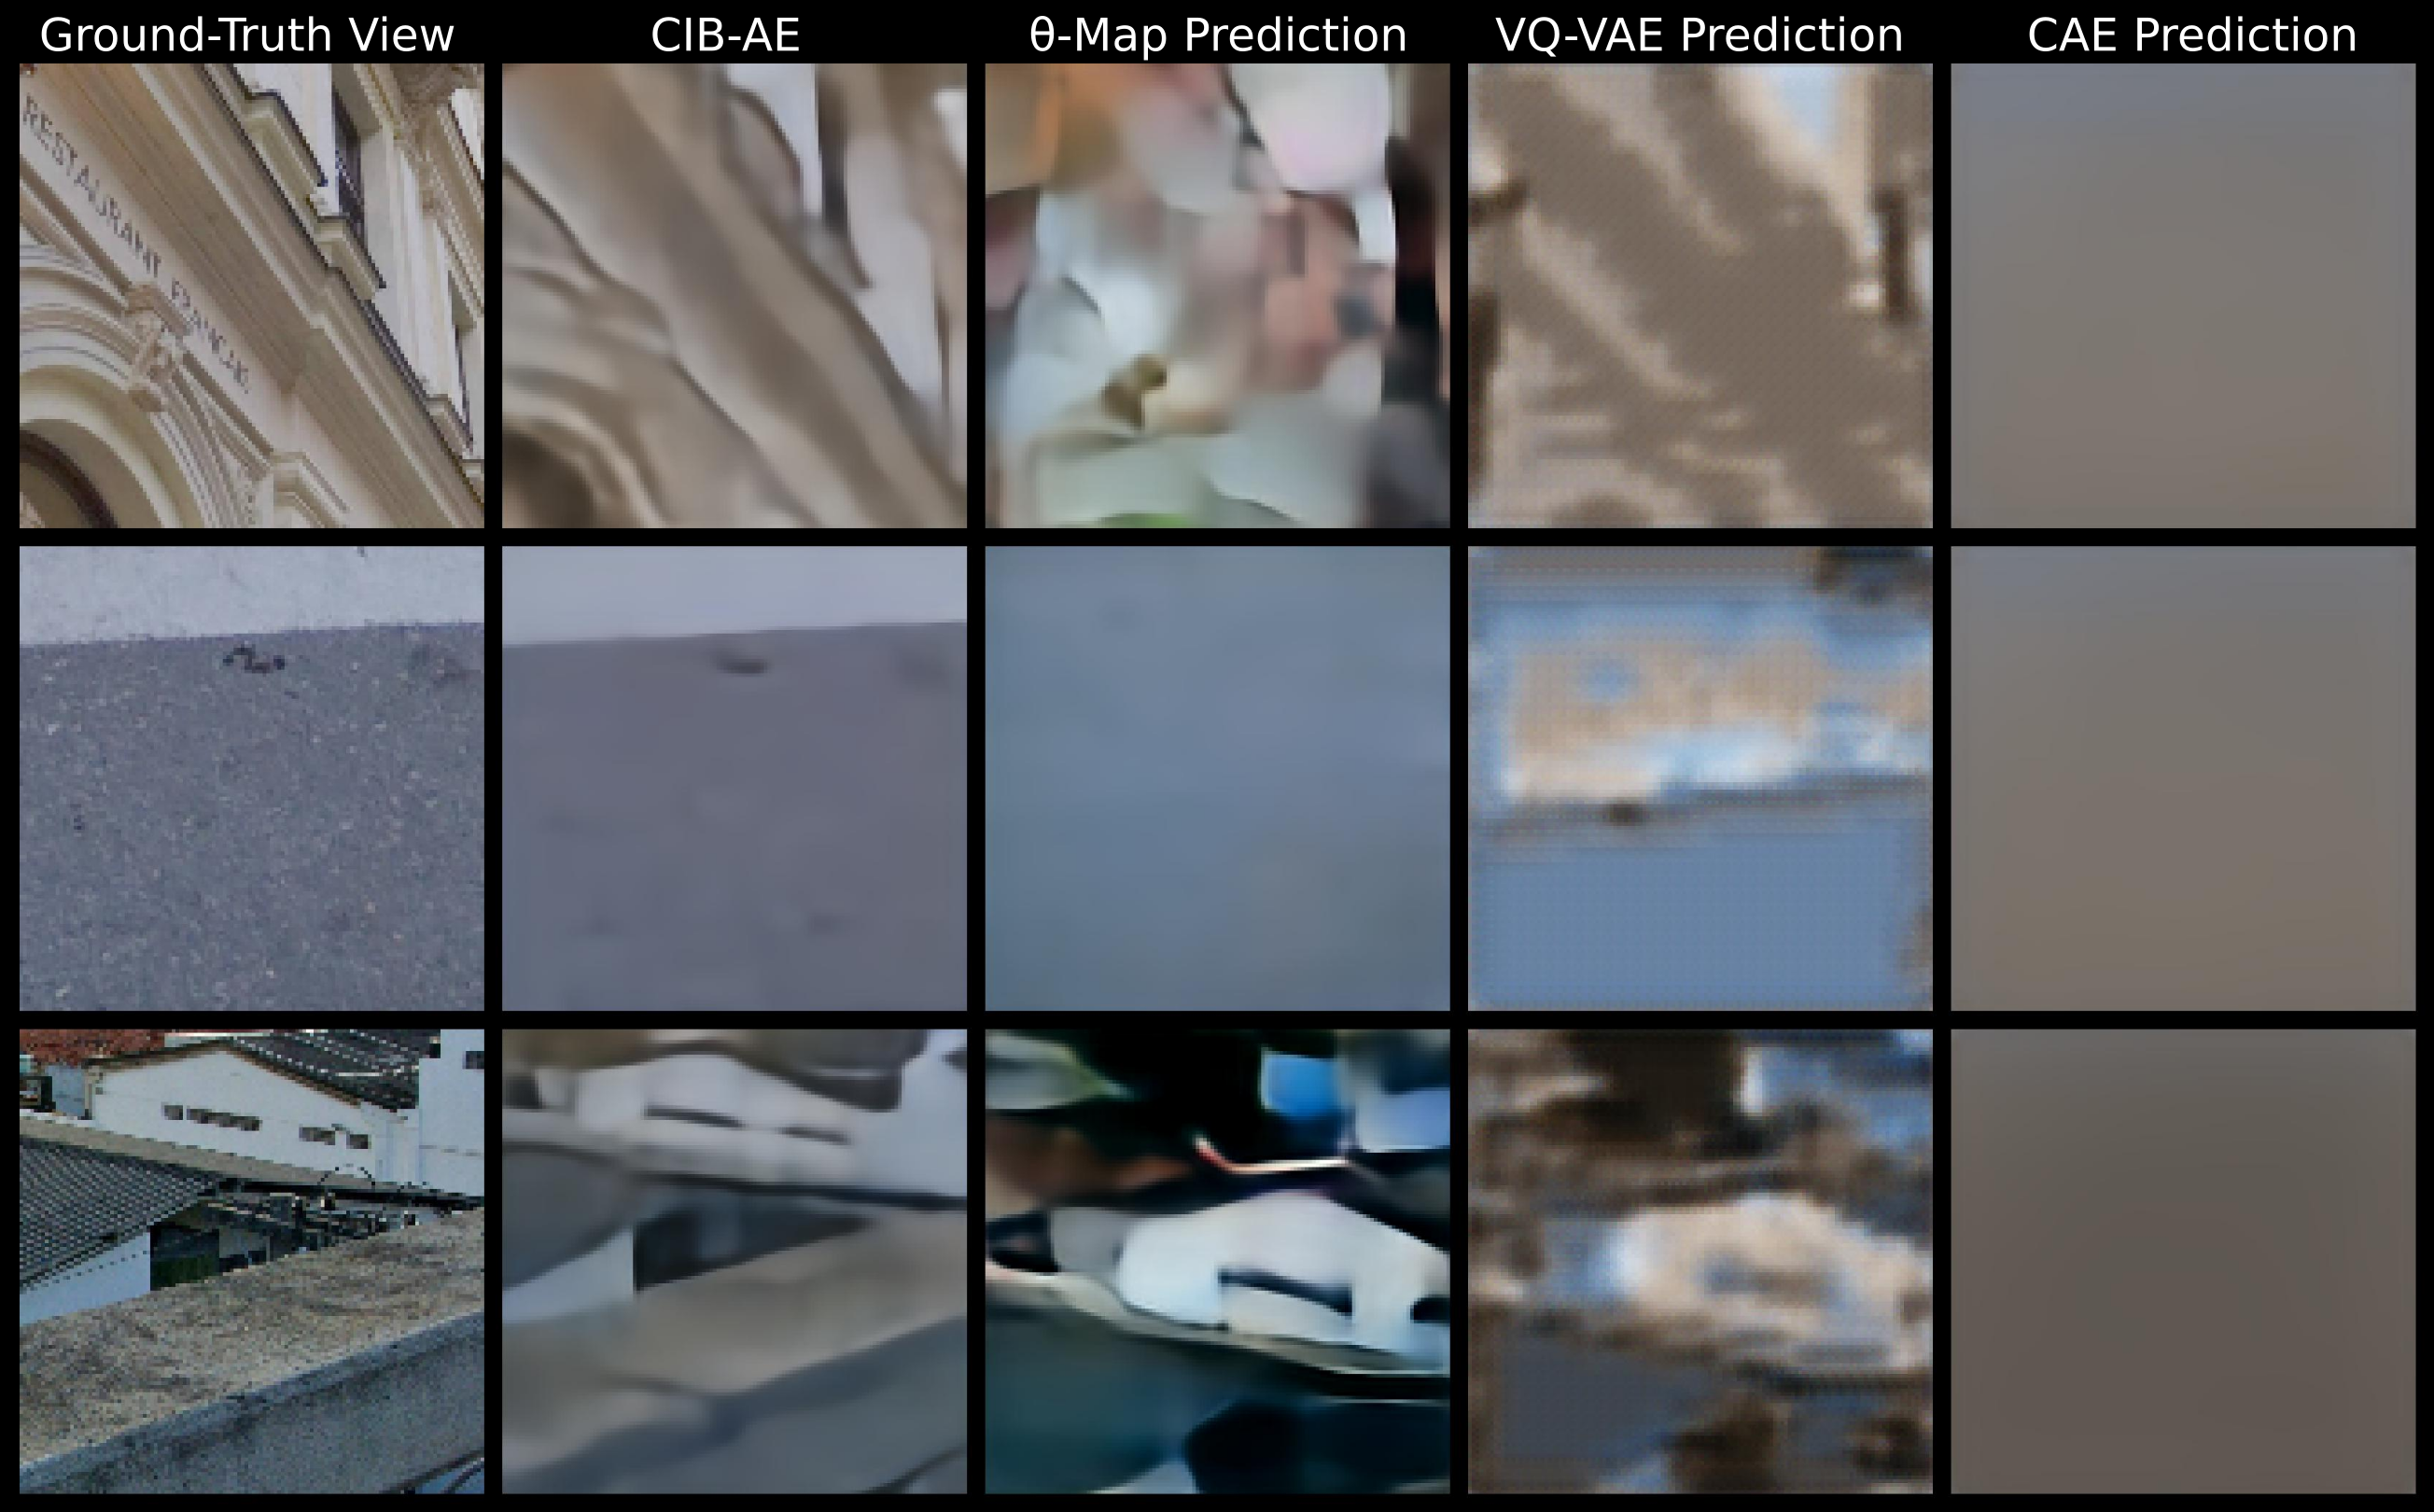
\includegraphics[width=0.89\columnwidth]{figures/ptz/test_stacked_intext.png}
        \label{fig:encoding-pred-strip}
    }
    \end{center}
    \caption{Observed \protect\subref{fig:encoding-obs-strip} and predicted encodings \protect\subref{fig:encoding-pred-strip} for random views from SUN360/street. From left to right the columns represent true image, CIB-AE autoencoding, topic prediction autoencoding, VQ-VAE latent prediction autoencoding, and plain CAE autoencoding. Many more examples are found in App.~\ref{ch:app-predictions}).
    }
    \label{fig:encoding-strip}
\end{figure}

Fig.~\ref{fig:vs_vqvae} shows the RMSE for observed topic encodings and predicted topic priors compared to the real images at the corresponding views. The low extent of the CAE RMSE whisker reveals that the conservative collapsed strategy of consistently predicting uniform grayish images is not necessarily bad in terms of pure pixel error, drawing out an important flaw of the pixel error as a performance measure at this level of compression. Nevertheless, to the extent that the RMSE distributions measure performance in our view prediction task, the data confirm our qualitative assesment that our method performs approximately as well as the VQ-VAE on average. Further, the more colorful, highher contrast images produced by our method are reflected by its higher variance than the more conservative VQ-VAE approach which tends to encode roughly the right shape, but obscure much of the color and texture.

\todo[inline]{Probably need more discussion here, possibly acknowledging limitations more head-on}

\begin{figure}
    \begin{center}
    \subfloat[]{
        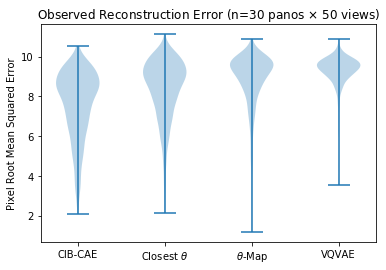
\includegraphics[width=0.48\columnwidth]{figures/ptz/vs_vqvae_obs.png}
        \label{fig:vs_vqvae_obs}
    }%
    \subfloat[]{
        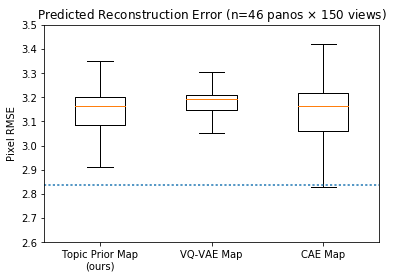
\includegraphics[width=0.48\columnwidth]{figures/ptz/vs_vqvae_pred.png}
        \label{fig:vs_vqvae_pred}
    }
    \end{center}
    \caption{ Performance comparison of our topic prior map with a VQ-VAE and a standard CAE.
    \protect\subref{fig:vs_vqvae_obs} Reconstruction performance for observed images (held out of training),
    \protect\subref{fig:vs_vqvae_pred} View prediction performance after training. The dashed line shows the median reconstruction error of the CIB-AE on this dataset. The box in this plot represents the interquartile range, while the whiskers represent the range of typical data (1.5 times IQR). RMSEs are computed for each image with respect to pixel values in the range [0,255].
    }
    \label{fig:vs_vqvae}
\end{figure}

\subsection{Visual topic-mixture search}
A second outcome of our work is a tool for exploring views in an environment through mixtures of topics. By directly decoding the topics, we are able to visually present a summary of the scene. Then, by providing an interface to specify a mixture of these topics, and performing a search within the topic-prior map, we enable a unique interaction that enables a user to visually explore an environment, as well as the information encoded by the topic model and the topic-prior map.

\begin{figure}
    \centering
    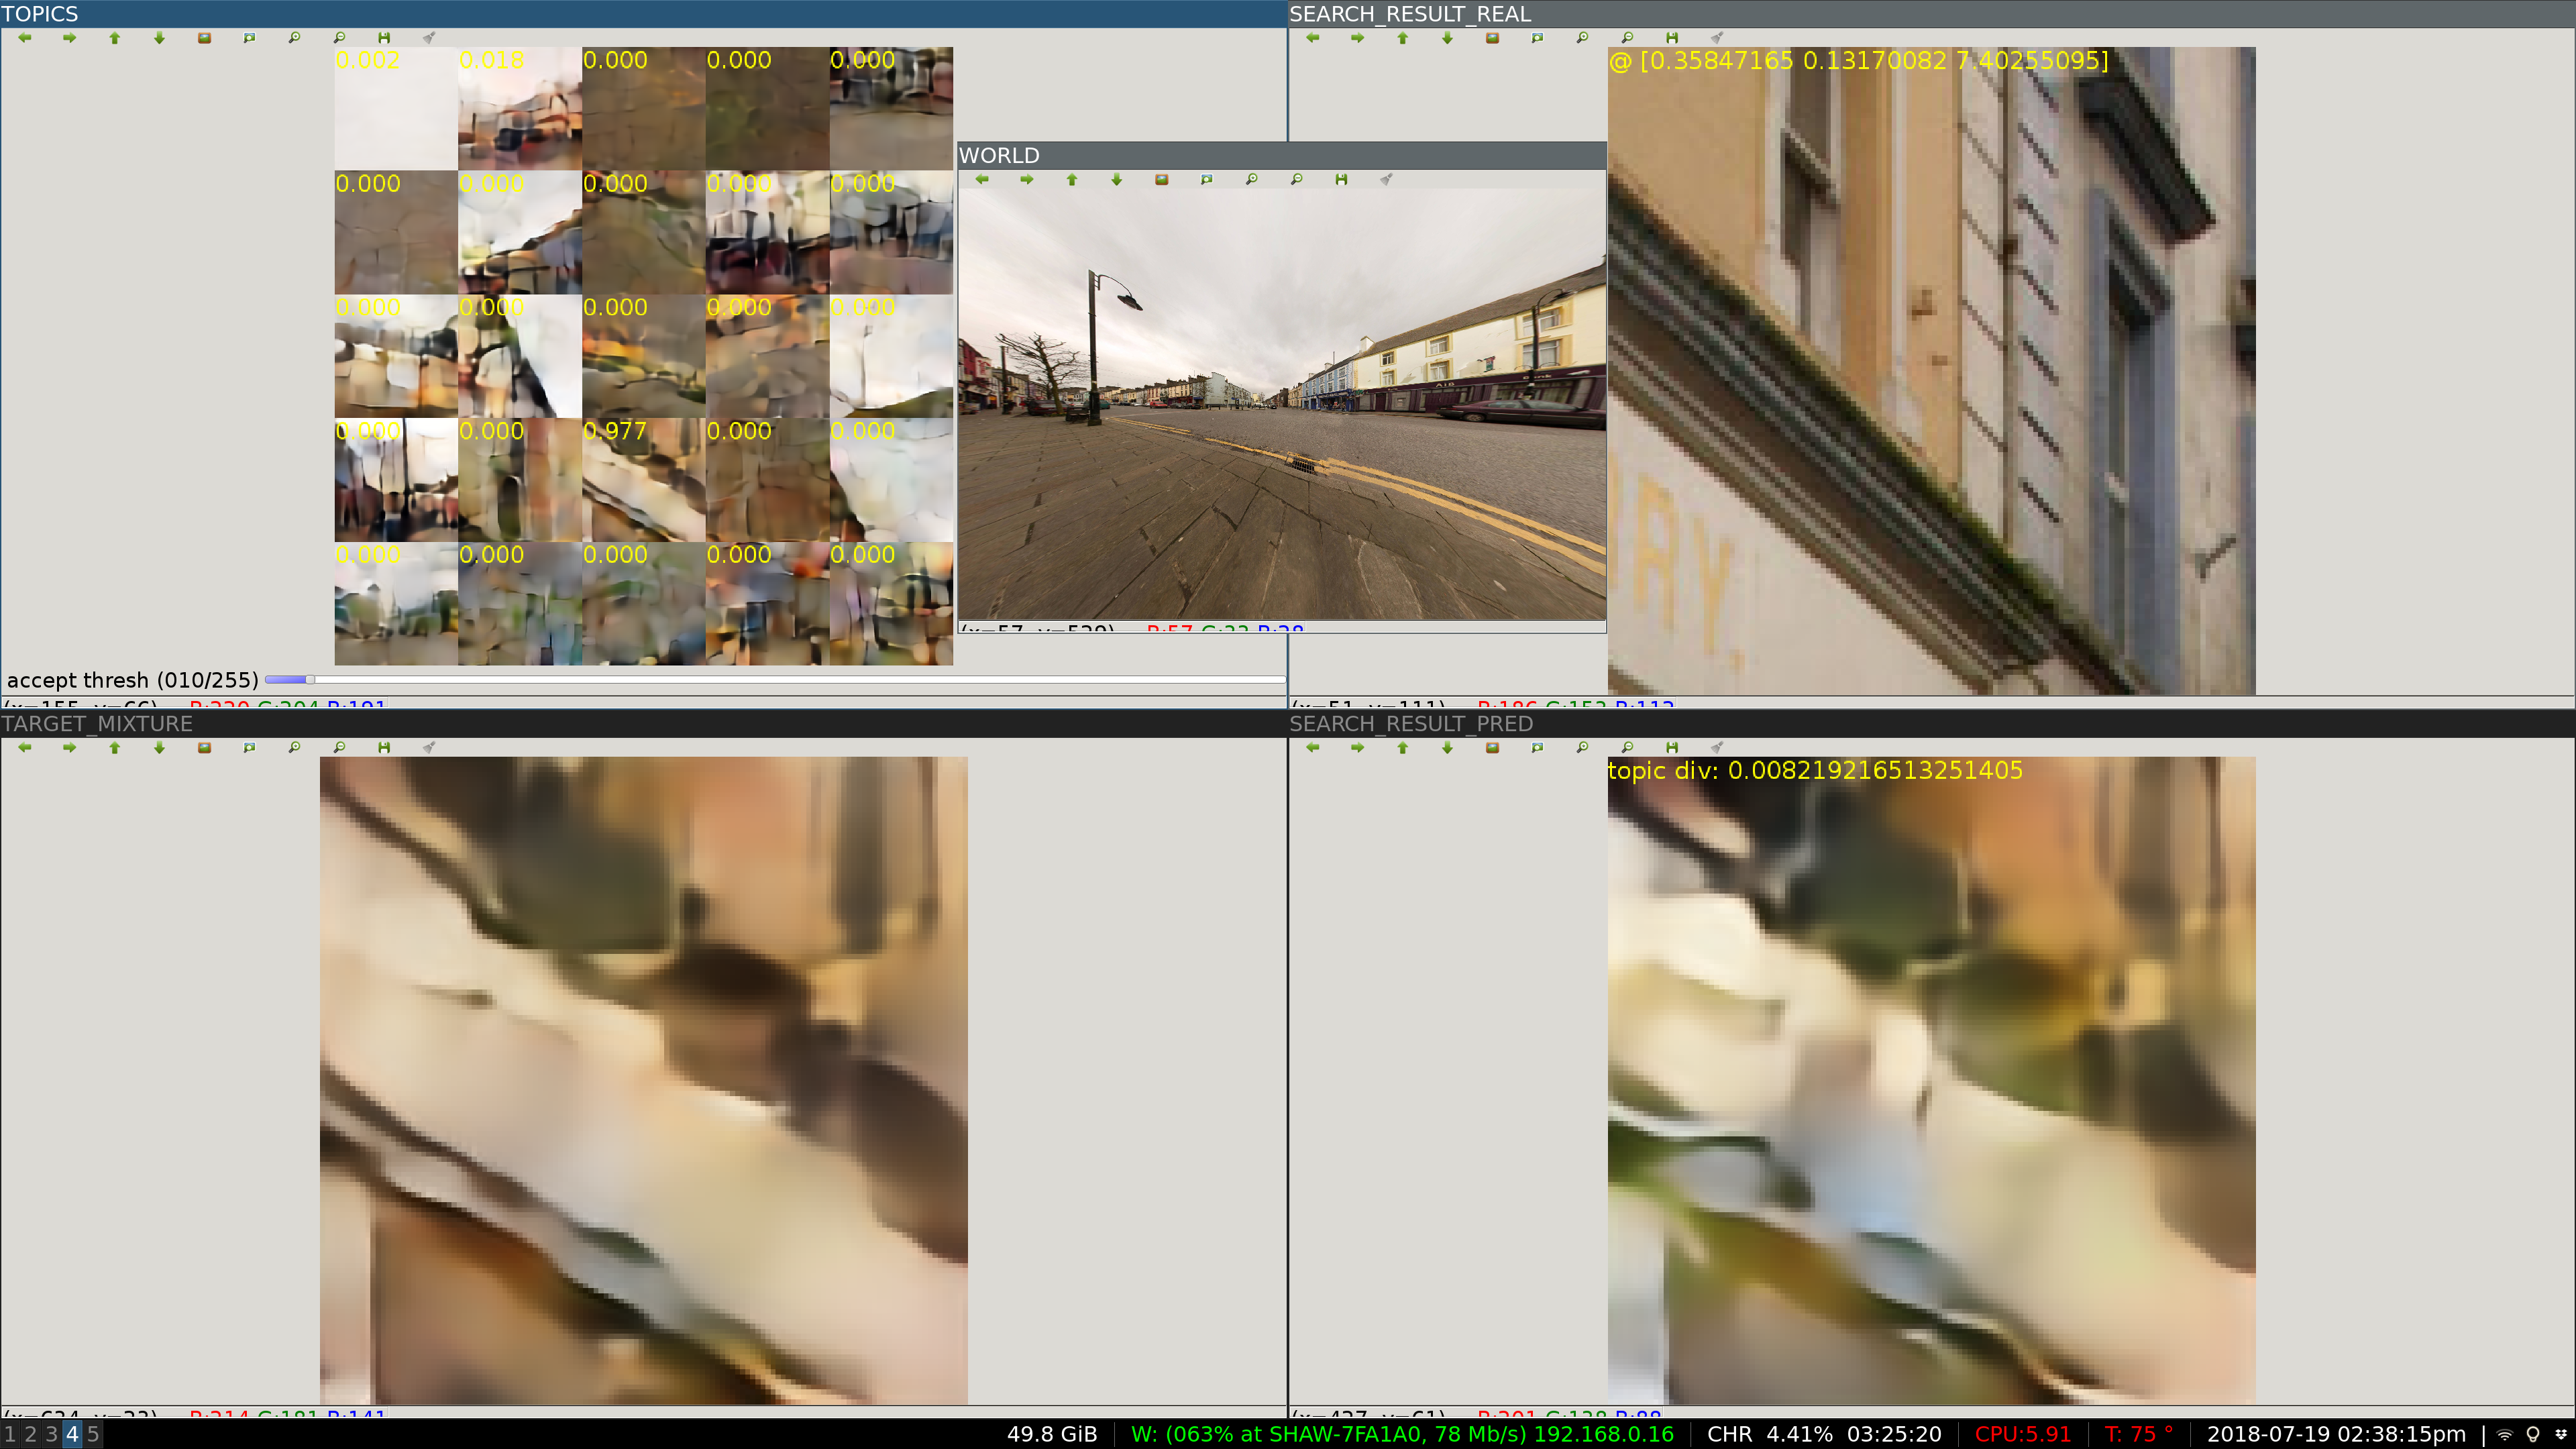
\includegraphics[width=\textwidth]{figures/ptz/interaction.png}
    \caption{Screenshot of visual topic-mixture search interaction. Counter-clockwise from Top-left: Direct decodings of 25 topics; numbers in each decoded topic indicate the proportion of the target mixture given to that topic. Decoding of the target-mixture. Sample from the view with the closest topic distribution given by our spatial prediction model: topic div gives the divergence between the predicted encoding and the target encoding. True image at the closest topic distribution. Demo video at \url{http://cim.mcgill.ca/~akalmbach/thesis/demos.html}}
    \label{fig:interaction}
\end{figure}

\section{Discussion}

\subsection{Active learning}\label{sec:active-learning}
As a complimentary task to learning the view prediction model, we also spent significant effort on the problem of \emph{efficiently} learning the view prediction model, that is, trying to accurately predict views in novel locations with as few training observations as possible. Although the specific model is novel, there is a rich literature on active learning (well summarized by \citep{settles2012active}), including many applications of efficient spatial sampling strategies drawing from the Gaussian Process (GP) models of \citep{Seo2000,guestrin2005near}. Recent work has touched on applications very similar to ours, such as determining where to take images to build a mosaic using a GP-based approach \citep{sandeep_crv_2016}, and which cells in a `view-grid' to observe to be able to predict the rest using a deep reinforcement learning based approach \citep{Jayaraman2017}.

We experimented with using GP-based upper confidence bounds on both the cross-entropy $H\left[e(I_x) \| \theta_x\Phi \right]$ and encoding divergence $D_{KL}\left[e(I_x)_x \| \theta_x\Phi\right]$ as well as using the predicted topic-prior entropy $H\left[\theta(x)\right]$ from our model as acquisition functions determining the best sample location given the set of previously observed ones. We applied these acquisition functions to both the view-prediction problem and training a supervised classifier, however found that neither outperformed a uniform sampling strategy. We did observe that these policies resulted in more observations of complex images as opposed to simple ones (such as all blue sky or gray asphalt), however spending more time learning from complex examples did not improve performance as measured by pixel MSE. It is our hypothesis that this was caused by a combination of biasing the topic model to use all its topics to describe a few small parts of the image (\emph{eg.} the cross-entropy method was very attracted to leaves if they were in the scene), and the limitations of MSE as a performance measurement for images with complex textures.

\subsection{MAP vs MLE topic estimates}

\subsection{Getting more from geometry and training other feature function}
Of note is the level of performance our model is able to achieve with a very simplistic geometric model. We use a Euclidean distance to place a prior on the similarity between views in both the topic model and the spatial prediction model. Clearly, however, there is more information to be gained from geometry in this problem. For instance, our feature does contain spatial information, so an edge in one location and the same edge translated or rotated to another location do not necessarily have similar encodings. This means that the natural categories in a panorama may need to be described by multiple very location specific topics with our model. Further, the spatial prediction model could benefit from more sophisticated geometry. A similar operation to our projection of rectangular panorama images to rectified views could be used to ensure that training images are used to fill in information for all overlapping views. Even the simplpest case of upsampling the center of a wide fov image to get information about a more zoomed in view would significantly improve our predictions.

\subsection{End-to-End Variational LDA Autoencoder}
While the CIB-AE provides a slight modifications that can be made to many standard networks to produce encodings roughly compatible with the Dirichlet prior of LDA, it is natural to ask whether the full model can be learned end-to-end, and fine-tuned for particular environments instead of training a separate model. In fact, \citep{srivastava2017autoencoding} explores implementing the LDA prior for the latent space of a Variational autoencoder, and although the Dirichlet distribution resists exact reparameterization with a simple distribution as is used in other Variational autoencoders, they use a Laplace approximation to achieve comparable results to the standard mean-field variational approximation with much more flexibility. Although the extra dependencies in the spatio-temporal topic model are not compatible with the reparameterization used, we envision pre-training an LDA inference network similar to \citet{srivastava2017autoencoding} similar to our CIB-AE training procedure, and then using the resulting word encoder-decoder along with the Gibbs sampler spatio-temporal topic model, which could be initialilzed from the learned $\Phi$ matrix of the non-spatial topic model.